%%%%%%%%%%%%%%%%%%%%%%%%%%%%%%%%%%%%%%%%%%%%%%%
%%% Template for lab reports used at STIMA
%%%%%%%%%%%%%%%%%%%%%%%%%%%%%%%%%%%%%%%%%%%%%%%

%%%%%%%%%%%%%%%%%%%%%%%%%%%%%% Sets the document class for the document
% Openany is added to remove the book style of starting every new chapter on an odd page (not needed for reports)
\documentclass[10pt,swedish, openany]{book}

%%%%%%%%%%%%%%%%%%%%%%%%%%%%%% Loading packages that alter the style
\usepackage[]{graphicx}
\usepackage[]{color}
\usepackage{alltt}
\usepackage[T1]{fontenc}
\usepackage[utf8]{inputenc}
\setcounter{secnumdepth}{3}
\setcounter{tocdepth}{3}
\setlength{\parskip}{\smallskipamount}
\setlength{\parindent}{0pt}
\usepackage{amsmath}
\usepackage{amssymb,latexsym}
\usepackage{mathtools}
\usepackage{subcaption}


% Set page margins
\usepackage[top=100pt,bottom=100pt,left=68pt,right=66pt]{geometry}

% Package used for placeholder text
\usepackage{lipsum}

% Prevents LaTeX from filling out a page to the bottom
\raggedbottom

% Adding both languages, Swedish and English, so they can be used intermittently in for example abstracts.
\usepackage[swedish, english]{babel}

% All page numbers positioned at the bottom of the page
\usepackage{fancyhdr}
\fancyhf{} % clear all header and footers
\fancyfoot[C]{\thepage}
\renewcommand{\headrulewidth}{0pt} % remove the header rule
\pagestyle{fancy}

% Changes the style of chapter headings
\usepackage{titlesec}
\titleformat{\chapter}
   {\normalfont\LARGE\bfseries}{\thechapter.}{1em}{}
% Change distance between chapter header and text
\titlespacing{\chapter}{0pt}{50pt}{2\baselineskip}

% Adds table captions above the table per default
\usepackage{float}
\floatstyle{plaintop}
\restylefloat{table}

% Adds space between caption and table
\usepackage[tableposition=top]{caption}

% Adds hyperlinks to references and ToC
\usepackage{hyperref}
\hypersetup{hidelinks,linkcolor = black} % Changes the link color to black and hides the hideous red border that usually is created

% If multiple images are to be added, a folder (path) with all the images can be added here 
\graphicspath{ {images/} }

% Separates the first part of the report/thesis in Roman numerals
\frontmatter

% add some useful definitions
\def\MeV{\ifmmode {\mathrm{\ Me\kern -0.1em V}}\else
                   \textrm{Me\kern -0.1em V}\fi}%  

\def\GeV{\ifmmode {\mathrm{\ Ge\kern -0.1em V}}\else
                   \textrm{Ge\kern -0.1em V}\fi}%  

%%%%%%%%%%%%%%%%%%%%%%%%%%%%%% Starts the document
\begin{document}

%%% Selects the language to be used for the first couple of pages
\selectlanguage{english}

%%%%% Adds the title page
\begin{titlepage}
	\clearpage\thispagestyle{empty}
	\centering
	\vspace{2cm}

	% Titles
	{\large  \par}
	\vspace{8cm}
        {\Huge \textbf{Parity Violation in $\beta$ desintegrations}} \\
	\vspace{1cm}
	{\large \textbf{Laboratoire IV} \par}
	\vspace{2cm}
	{\large Luiza Adelina Ciucu \\ % \\ specifies a new line
	             Ana Ventura Barroso \par}
	\vspace{4cm}

    
\includegraphics[scale=0.75]{logo.jpg}
    
    \vspace{4cm}
    
	% Information about the University
	{\normalsize Universit\'e de Gen\`eve \\ 
		Facult\'e de Sciences \\
		Section de physique \\
		D\'epartement de Physique Nucl\'eaire et Corpusculaire \par}
		
	% Set the date
	{\normalsize 29-10-2019 \par}
	\vspace{2cm}
	
	\pagebreak

\end{titlepage}

% Adds a table of contents
\tableofcontents{}

\clearpage

\listoffigures

\clearpage


%%%%%%%%%%%%%%%%%%%%%%%%%%%%%%%%%%%%%%%%%%%%%%%%%%%%%%%%%%%%%%%%%%%%%%%%%%%%%%%%%%%%%%%%%%%%
%%%%%%%%%%%% The rows above should not be changed except for the title page information
%%%%%%%%%%%%%%%%%%%%%%%%%%%%%%%%%%%%%%%%%%%%%%%%%%%%%%%%%%%%%%%%%%%%%%%%%%%%%%%%%%%%%%%%%%%%
%%%%% Text body starts here!
\mainmatter

\chapter{Introduction}
\label{chapter:Introduction}

``Nowadays, with broken symmetry almost universally accepted as a way of life, it is perhaps difficult for a modern student in physics to realize the basic taboo of the past period. Thirty years ago, it was unthinkable (certainly to me) that anyone should question the validity of symmetries under space inversion, charge conjugation and time reversal. It would have been almost sacrilegious to test such \emph{unholy} thoughts. [...]'' \cite{violation}. \\

This was spoken by Robert Novick during the symposium at the University of Columbia in 1986. They were celebrating 30 years since the discovery of parity violation. Indeed, these words are real. In the university we learn since the beginning that some symmetries are broken and this fact is totally necessary to explain physics. As physicists we love symmetry. Therefore, even if now the concept of symmetry breaking is well established, it must have been really hard to even consider this concept in the beginning.\\

In 1918, Emmy Noether formalised the relation between conservation laws and symmetries. In classic mechanics, the space-time symmetries refer to energy, momentum and angular momentum conservation. In quantum mechanics and particle physics, the right-left symmetry gives rise to the parity conservation. This law of parity conservation was widely considered true. There was no theoretical reason why all four fundamental particle interactions would conserve this parity. Indeed, it turns out that the weak interaction does violate parity. \\

The parity violation for the weak interactions was proposed theoretically in 1956 by T.D. Lee and C.L. Yang, and confirmed experimentally by Chien-Shiung Wu the same year. How did they arrive to their ideas? In 1956, this law of parity conservation started to raise doubts. Lee and Yang from Columbia University in the USA decided to run an experiment to validate the idea of the parity violation in weak interactions. ``To decide unequivocally whether parity is conserved in weak interactions, one must perform an experiment to determine whether weak interactions differentiate the right from the left.'' \cite{parity}. This idea lead Lee and Yang to design an experiment for testing their hypothesis. They requested the help of Chien-Shiung Wu, one of the world expert in the $\beta$ disintegration. Together they figured out the famous experiment of the polarisation of Cobalt 60, which confirmed indeed the Lee and Yang theory. Later the experiment was refined by Frauenfelder and his group in 1957 \cite{paritos}. \\

The goal of the lab and this report is to reproduce Frauenfelder and demonstrate experimentally parity violation. A radioactive source suffers beta decay of a neutron decaying to a proton, an electron and an anti-neutrino. The emitted electrons are scattered against a polarised iron foil. The relative polatisation of the source and target electrons affects the process cross section. We will show that the source electrons emitted in the weak decay have a preferred polarisation. \\

The report is structured as follows. In Chapter~\ref{chapter:TheoreticalAspects} the theoretical aspects of the weak interaction and of the Moeller scattering are discussed. In Chapter~\ref{chapter:ExperimentalSetup} the experimental setup is described, with the radioactive source, the photomultiplier tubes and the electronics. Chapter~\ref{chapter:Calibration} presents the calibration of the experiment, the foil polarisation, and the measurements obtained. Chapter~\ref{chapter:DataAnalysis} presents the interpretation of the measurements, while Chapter~\ref{chapter:Conclusion} concludes the report. 

\chapter{Theoretical aspects}
\label{chapter:TheoreticalAspects}

% A * after the section/chapter command indicates an unnumbered header which will not be added to the table of contents
\section{Weak interactions and parity}

\subsection{Parity transformation}
A parity transformation represents the inversion in the sign of the spatial coordinates, while time remains unchanged, namely $(t,x) \rightarrow (t,-x)$, as illustrated in Figure~\ref{fig:parity}.
\begin{figure}[h]
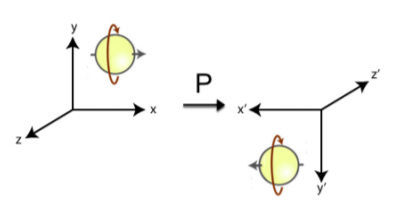
\includegraphics[scale=1]{parity.png}
\centering
\caption{Parity transformation.}
\label{fig:parity}
\end{figure}

True vectors, such as momentum, change sign under the parity transformation, while scalars, such as angular momentum, are invariant. Also under this transformation, scalars, such as energy, remain invariant, while pseudo-scalars, such as helicity, change sign.\\

The parity transformation has also an effect on particles' wave functions. Left-handed particles transform into right-handed particles, and vice-versa, because the spin operator is a pseudo-vector.\\

The electromagnetic and strong interactions are invariant under the parity transformation, with only the weak interaction violating it.\\

\subsection{Field theory}

For understanding better the effect of the parity transformation, several concepts of field theory have to be introduced.\\

Quantum field theory is a synthesis of quantum mechanics and special relativity. Quantum mechanics is intrinsically a non-relativistic theory, where particles are described by wave functions. When including special relativity, instead of thinking of particles in an external classical potential, one identifies particles with the modes of a field. Thus the Lorentz symmetry is implemented. Particle representations are invariant under the Lorentz transformation and follow a SU(2) symmetry.\\

In this context, we introduce the spinorial representation, one of the fundamental representation of SU(2) group. As such, with spin-1/2 particles it is possible to build composite systems with all possible integer or half-integer spin values.\\

We define the right-handed Weyl spinor, $\psi_R$, and the left-handed Weyl spinor, $\psi_L$, 

\begin{equation}
    \psi_L = (\frac{1}{2},0), 
\end{equation}
\begin{equation}
    \psi_R = (0,\frac{1}{2}).
\end{equation}

We know experimentally that parity is violated by the weak interaction. Theoretically this is reflected by the fact that right- and left-handed components of the spin-1/2 particles enter the theory in a very different way (through the $V-A$ structure). However at sufficiently low energies, the effect of the weak interactions is small. The dominant contributions come from electromagnetic and strong interactions, where parity is conserved. In this case we need to introduce the Dirac field, which provides a representation of the Lorentz and parity transformation,
\begin{equation}
    \Psi = \psi_R = (0,\frac{1}{2}).
\end{equation}

\subsection{V-A structure}

To find out if parity is conserved in an interaction, the parity transformation is applied to the current interaction vertex. For quantum electrodynamics (QED) and quantum chromodynamics (QCD), the form of the interaction vertex is $j^{\mu}=\bar{u}(p')\gamma^{\mu}u(p)$, is that of a vector, so it will change sign under the parity transformation. Since the interaction matrix element is composed of two currents, the negative signs cancel each other and parity is conserved.\\

Due to the fact that weak interaction violates parity, we can assume that the current interaction vertex is not of the same form as that of the QED and QCD currents. The Lorentz invariant requirement restricts the form of the interaction to covariant bilinear combinations of two spinors. The most general form for the interaction between a boson and a fermion with the exchange of a spin-1 boson is a linear combination of vector and axial vector currents, 
\begin{equation}
    j^{\mu} \propto g_V j^{\mu}_V + g_A j^{\mu}_A, 
\end{equation}

where $g_v$ and $g_A$ are vector and axial vector coupling constants, respectively. Thus, the weak interaction has two components. One violates parity and the other conserves parity. The relative strength of the parity violating part compared to the parity conserving part is given by

\begin{equation}
    \alpha = \frac{g_V \cdot g_A}{g^2_V + g^2_A}.
\end{equation}

If one of the coupling constants is zero, parity is conserved. Maximal parity violation happens when $|g_V|=|g_A|$. Experiments confirm that the structure of the weak charged current is a vector minus the axial vector ($V-A$), with this vertex factor being given by
\begin{equation}
    \frac{- i g_W}{\sqrt{2}}\frac{1}{2}\gamma^{\mu}(1-\gamma^5).
\end{equation}

\subsection{Parity violation of the weak interaction}

Since the $W^{\pm}$ bosons are electrically charged, only they can exchange charge via the charge current interaction, as illustrated in Figure~\ref{fig:WInteraction}.
  
\begin{figure}[h]
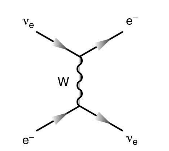
\includegraphics[scale=0.8]{charged.png}
\centering
\caption{Feynman Diagram for the charged current interaction.}
\label{fig:WInteraction}
\end{figure}  
  
Let's consider the interaction Lagrangian for the weak charged interactions
\begin{equation}
    L_{\rm CC} = g_W(W^+_{\mu}J^{+ ,\mu} + W^-_{\mu}J^{- ,\mu}),
\end{equation}

where the charge-raising current operator and the charge-lowering operator are given by
\begin{equation}
    J^+ = \frac{1}{\sqrt{2}} \sum_l (\bar{\nu_l}\frac{\gamma^{\mu}(1-\gamma^5)}{2}l) + \sum_q (\bar{q'}\frac{\gamma^{\mu}(1-\gamma^5)}{2}q),
\end{equation}

\begin{equation}
    J^- = \frac{1}{\sqrt{2}} \sum_l (\bar{l}\frac{\gamma^{\mu}(1-\gamma^5)}{2}\nu_l) + \sum_q (\bar{q}\frac{\gamma^{\mu}(1-\gamma^5)}{2}q').
\end{equation}

The sum over $l$ is the sum over the leptons, and the sum over $q$ is the sum over the quarks, where $q=(u,c,t)$ are the quark mass eigenstates and $q'=(d',s',b')$ are the flavor eigenstates, which are also the weak interaction eigenstates of the Cabbibo-Kobayashi-Maskawa matrix.\\

The left-handed projector operator is described by $P_{\rm L}=\frac{1}{2}(1-\gamma^5)$. This implies that the weak charged currents couple only  left-hand particles with right-hand antiparticles, and that parity is violated the most in the charged weak interaction. \\

The $Z^0$ boson is neutral (no electric charge). Thus it is the mediator of neutral current interaction, as illustrated in the Figure~\ref{fig:ZInteraction}. The interaction Lagrangian for the weak neutral interactions is given by
\begin{equation}
    L_{\rm NC} = \frac{g_W}{\cos{\theta_W}}J^{\mu}_Z Z_{\mu}.
\end{equation}

\begin{figure}[h]
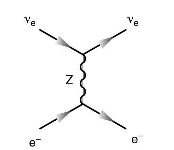
\includegraphics[scale=0.8]{neutral.png}
\centering
\caption{Feynman Diagram for neutral current interaction.}
\label{fig:ZInteraction}
\end{figure}  

Thus the neutral current is
\begin{equation}
    J_Z = \sum_j \bar{\psi_j}\gamma^{\mu} (\frac{(1-\gamma^5)}{2}T^3 - 2\sin^2{\theta_W}Q_j), 
\end{equation}

where the $T^3$ and Q are the weak isospin and the charge of the particle, respectively. $\theta_W$ represents the rotation due to the spontaneous symmetry breaking, or in other words thus the angle between the particles that are mass eigenvalues and the ones that are weak eigenvalues.\\

We take into consideration both the charged current (CC) and neutral current (NC), whose invariant amplitudes are given by
\begin{equation}
    i M_{\rm CC} = (-i g_W)^2 J^{\mu}_+ [\frac{-i}{q^2-M^2_W}(\eta_{\mu\nu}-\frac{q_{\mu}q_{\nu}}{M^2_W})] J_{- \mu},
\end{equation}
\begin{equation}
    i M_{\rm NC} = (\frac{-i g_W}{\cos{\theta_W}})^2 J^{\mu}_Z [\frac{-i}{q^2-M^2_Z}(\eta_{\mu\nu}-\frac{q_{\mu}q_{\nu}}{M^2_Z})] J_{Z \mu}.
\end{equation}

\subsection{Fermi theory}

Nevertheless, most of the interactions take places at low energies (on the order of a few \GeV). Since the masses of the  $W^\pm$ ($\approx 80 \GeV$) and $Z^0$ ($\approx 91 \GeV$) bosons dominate the kinematics of the propagator, we can assume the approximation $|q^2| << M^2_W$, which allows to describe weak interactions as low-energy effective theory. \\

For example, in our experiment the source electrons are obtained from a radioactive source via beta disintegration of a neutron ($n \rightarrow p e^- \bar{\nu_e}$). The energy involved is equal to the mass difference between the neutron and the proton, $\Delta m = m_n - m_p \approx 1.3 \MeV$. This is much smaller than the mass of the $W^\pm$  boson, which implies that the beta disintegration can be described by a low-energy effective theory. It is called the Fermi theory, since it was introduced by Enrico Fermi to explain the neutron disintegration . It assumes a 4-point direct interaction between the neutron proton, electron and neutrino, without involving any $W^\pm$ or  $Z^0$ boson, as illustrated in Figure~\ref{fig:PointLikeInteraction}. \\

\begin{figure}[h]
\includegraphics[scale=0.5]{Fermi.png}
\centering
\caption{Point like interaction.}
\label{fig:PointLikeInteraction}
\end{figure}  

Continuing the previous calculation, we express the $W$-boson propagator as

\begin{equation}
    \frac{-i}{q^2-M^2_W}(\eta_{\mu\nu}-\frac{q_{\mu}q_{\nu}}{M^2_W}) \rightarrow \frac{i \eta_{\mu\nu}}{M^2_W}.
\end{equation}

The effective interaction has no longer a $q^2$ dependence. Physically this corresponds to replacing the propagator with an interaction which occurs at a single point in space-time, or in other words with a point-like interaction, as illustrated in Figure~\ref{fig:PointLikeInteraction}.\\

For a general leptonic interaction the invariant amplitude is reduced to
\begin{equation}
    i M_{\rm CC} = \frac{- i g_W^2}{8M_W^2}[\bar{\nu_l}\gamma^{\mu}(1-\gamma^5)l][\bar{l}\gamma^{\mu}(1-\gamma^5)\nu_l], 
\end{equation}

where the relation between the weak interaction coupling constant and the coupling Fermi constant is given by
\begin{equation}
    \frac{G_F}{\sqrt{2}} = \frac{g_W^2}{8 M_W^2}.
\end{equation} 

Therefore, the interaction term in the effective theory Lagrangian is given by
\begin{equation}
L = \frac{-G_F}{\sqrt{2}}(j^{+,\mu} j^-_{\mu}),
\end{equation}

where $j = 2\sqrt{2} J$. \\

It is worth noting that the width of the process of the beta decay is not easy to compute, since the protons and neutrons involved are not free particles, but bound together inside nuclei, and themselves are also formed by bound states of quarks. Several approximations are needed. But the V-A structure of the interaction is maintained. 

\section{Moller Diffusion}

The goal of our experiment is to demonstrate the parity violation in the beta decay, which implies that there is a preference in the polarisation for the emitted electrons. Therefore we want to measure the emitted electron polarisations. The cross section of the electron-electron scattering, also called Moller scattering,  depends strongly on the polarisation. We then design our own experiment to scatter the emitted electrons against electrons from a target. In this section we will compute the polarised cross section for the Moller scattering.

\begin{equation}
    e^- + e^- \rightarrow e^- + e^-.
\end{equation}

In general, the Moller scattering process is described by four tree-level diagrams of neutral current: the two from QED, exchanging a photon ($\gamma$), and two from the weak interaction, exchanging a $Z^0$ boson, as illustrated in Figure~\ref{fig:MollerScattering}. The weak force is purely left-handed, but the weak and electromagnetic forces mix into the particles we observe. \\

\begin{figure}[h]
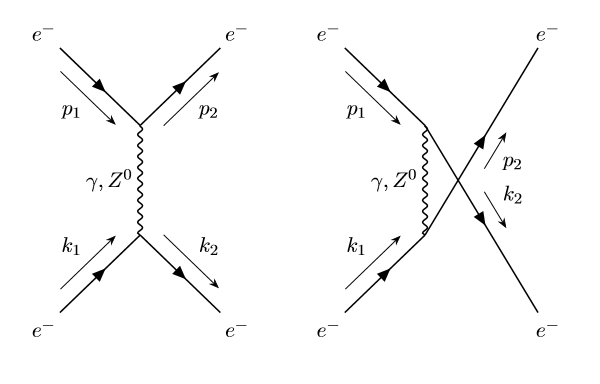
\includegraphics[scale=0.5]{moller.png}
\centering
\caption{t-channel and u-channel Feynman diagrams for the Moller scattering.}
\label{fig:MollerScattering}
\end{figure}

But in our experiment, the radioactive source is Strontium-90, which emits electrons with a maximum energy of 2.28 \MeV, as described in Chapter~\ref{chapter:ExperimentalSetup}. This energy is much smaller than the mass of the $Z^0$ boson. We can therefore ignore the contributions with the a $Z^0$ boson, and keep only the two contributions with the photon. A detailed calculation is presented below, first with all four Feynman diagrams and then with the remaining non-negligible two. The invariant amplitude of this process is given by

\begin{multline}
\\
     i\mathcal{M} = i\mathcal{M}^{\gamma}_{\rm t-channel} + i\mathcal{M}^{\gamma}_{\rm u-channel} + i\mathcal{M}^{Z}_{\rm t-channel} + i\mathcal{M}^{Z}_{\rm u-channel} =\\ [\bar{u}(k_2)(-ie\gamma^{\mu})u(k_1)][\frac{-i\eta_{\mu\nu}}{(k_1-k_2)^2}][\bar{u}(p_2)(-ie\gamma^{\nu})u(p_1)] -\\
    [\bar{u}(p_2)(-ie\gamma^{\mu})u(k_1)][\frac{-i\eta_{\mu\nu}}{(k_1-p_2)^2}][\bar{u}(k_2)(-ie\gamma^{\nu})u(p_1)] +\\
    (-i \frac{g_W}{\cos{\theta_W}})^2[\bar{u}(k_2)\frac{(\gamma^{\mu}(c_v - c_A\gamma^5)}{2}u(k_1)][\frac{-i(\eta_{\mu\nu}-\frac{(k_1-k_2)_{\mu}(k_1-k_2)_{\nu}}{M_Z^2})}{(k_1-k_2)^2-M_Z^2}][\bar{u}(p_2)\frac{(\gamma^{\mu}(c_v - c_A\gamma^5)}{2}u(p_1)] -\\
    (-i \frac{g_W}{\cos{\theta_W}})^2[\bar{u}(p_2)\frac{(\gamma^{\mu}(c_v - c_A\gamma^5)}{2}u(k_1)][\frac{-i(\eta_{\mu\nu}-\frac{(k_1-p_2)_{\mu}(k_1-k_2)_{\nu}}{M_Z^2})}{(k_1-k_2)^2-M_Z^2}][\bar{u}(k_2)\frac{(\gamma^{\mu}(c_v - c_A\gamma^5)}{2}u(p_1)].
\end{multline}

In our low-energy approximation, it is acceptable to neglect the process due to the weak interaction, and the invariant amplitude becomes

\begin{multline}
     i\mathcal{M} = [\bar{u}(k_2)(-ie\gamma^{\mu})u(k_1)][\frac{-i\eta_{\mu\nu}}{(k_1-k_2)^2}][\bar{u}(p_2)(-ie\gamma^{\nu})u(p_1)] -
    [\bar{u}(p_2)(-ie\gamma^{\mu})u(k_1)][\frac{-i\eta_{\mu\nu}}{(k_1-p_2)^2}][\bar{u}(k_2)(-ie\gamma^{\nu})u(p_1)] .
\end{multline}

Once the invariant amplitude is known, we can compute the cross section, which in the centre-of-mass is defined as

\begin{equation}
    \frac{d\sigma}{d\Omega} = \frac{1}{\pi^2}\frac{E_1^2E_2^2}{(E_1+E_2)^2} \sum_{\rm final \ spins} |\mathcal{M}|^2.
\end{equation}

We have to sum over all the spins in the final state, because we accept all the possible configurations. Note that we do not know the spin configurations of the electrons coming from the source. Measuring that is the goal of the experiment.

\subsection{Polarisation}

Since the process is a $\beta$ disintegration, the incoming (source) electrons are left-handed due to weak interaction structure. Thus they are longitudinally polarised.\\

When the target is placed inside a magnetic field, their spins of the electrons of the target are aligned with the field, so the target electrons are also longitudinal polarised.\\

Since both electrons are longitudinal polarised, we can have two different cross sections for two different spin configurations: parallel ($\sigma_{\leftleftarrows}$) or antiparallel ($\sigma_{\rightleftarrows}$) polarisations.\\

For describing the longitudinal polarisation, it is necessary to impose that the spinors $u_{\epsilon1}$ and $u_{\epsilon2}$ are eigenstates of the spin operator $\frac{1}{2}\Sigma = \sigma \frac{p}{|\vec{p}|}$, such that

\begin{equation}
\frac{1}{2}
   \begin{pmatrix}
   \vec{\sigma} && 0 \\
   0 && \vec{\sigma}
   \end{pmatrix} \cdot u_{\epsilon} = \epsilon \cdot u_{\epsilon} \quad \Rightarrow \quad \begin{matrix} u_{\epsilon 1} = \frac{1}{2} \Sigma_{\epsilon} (1+\epsilon_1 \sigma_1) u_{\epsilon}\\
   u_{\epsilon 2} = \frac{1}{2} \Sigma_{\epsilon} (1+\epsilon_2 \sigma_2) u_{\epsilon}
   \end{matrix}.
\end{equation}

Using the completeness relation ($\sum_{s=1,2} u^{(s)}(p) \bar{u}^{(s)}(p) =  \displaystyle{\not} p + m
$) and the notation above, we define the cross section as
\begin{equation}
    \frac{d\sigma}{d\Omega} = \frac{\alpha^2 E_1^2E_2^2}{(E_1+E_2)^2 E_1'E_2'} (\frac{\rm A}{(k_1 - k_2)^2} + \frac{\rm B}{(k_1 - p_2)^2} - \frac{\rm C+D}{(k_1 - k_2)^2(k_1 - p_2)^2}),
\end{equation}

where $\alpha$ is the fine structure constant, defined as $e^2/4\pi$. Also A and B are defined as 

\centerline{${\rm A} =  \frac{1}{16} Tr[(k_1+im_e)\gamma_{\mu}(1+\epsilon_1\sigma_{k1})(k_2+im_e)\gamma_{\nu}(p_1+im_e)\gamma^{\mu}(1+\epsilon_2\sigma_{p1})(p_2+im_e)\gamma^{\nu}]$,}

\centerline{${\rm B} = \frac{1}{16} Tr[(k_1+im_e)\gamma_{\mu}(1+\epsilon_1\sigma_{k1})(p_2+im_e)\gamma_{\nu}(p_1+im_e)\gamma^{\mu}(1+\epsilon_2\sigma_{p1})(k_2+im_e)\gamma^{\nu}]$,}

respectively. Furthermore, C and D are obtained from A and B, respectively, by exchanging $k_1$ for $p_1$.\\

We define the cross section with parallel and antiparallel initial spins, respectively, as illustrated in Figure~\ref{fig:ParallelAntiparallelPolarisation}.

\begin{figure}[h]
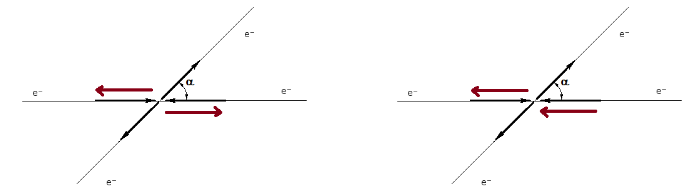
\includegraphics[scale=0.5]{polarisation.png}
\centering
\caption{Parallel and antiparallel polarisation.}
\label{fig:ParallelAntiparallelPolarisation}
\end{figure}

This implies that \\
        \centerline{parallel spins $\rightarrow \epsilon_1 = - \epsilon_2$, }\\
        \centerline{antiparallel spins $\rightarrow \epsilon_1 = \epsilon_2$.}
        
 Developing the traces and using the previous relation, in the centre-of-mass we obtain the following cross sections
 \begin{equation}
     \sigma_{\leftleftarrows} = \alpha^2 \frac{2\cos^2{\theta}+\beta^2(3\cos^2{\theta}+\cos^4{\theta})+\beta^4(1+\cos^4{\theta})}{2E^2\beta^4\sin^2{\theta}},
 \end{equation}
 
 \begin{equation}
     \sigma_{\rightleftarrows} = \alpha^2 \frac{1+\cos^2{\theta}+\beta^2(2+3\cos^2{\theta}-\cos^4{\theta})+\beta^4(5-4\cos^2{\theta}+\cos^4{\theta})}{2E^2\beta^4\sin^2{\theta}},
 \end{equation}
 
where $\beta$ is the ratio of the velocity and the speed of light, $\gamma$ is the Lorentz factor and $\theta$ is the diffusion angle.

\subsection{Asymmetry}
\label{asym}

We do not need to measure absolute cross sections, as it is easier to measure the asymmetry, defined as follows from the parallel and antiparallel cross sections, 

\begin{equation}\label{27}
    A = \frac{\sigma_{\rightleftarrows}-\sigma_{\leftleftarrows}}{\sigma_{\rightleftarrows}+\sigma_{\leftleftarrows}} = \frac{1-\cos^2{\theta}+\beta^2(2-2\cos^4{\theta})+\beta^4(4-5\cos^2{\theta}+\cos^4{\theta})}{1+3\cos^2{\theta}+\beta^2(2+6\cos^2{\theta})+\beta^4(6-3\cos^2{\theta}+\cos^4{\theta})},
\end{equation}

and illustrated as a function of $\beta$ and $\theta$ in Figure~\ref{fig:Asymmetry}.

\begin{figure}[h]
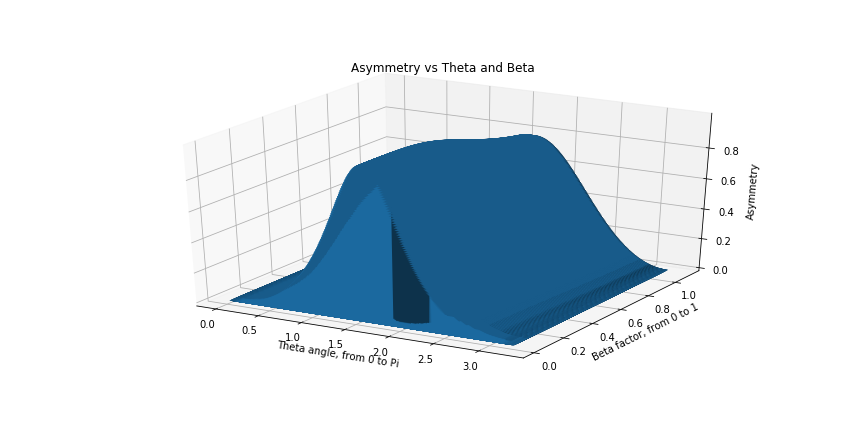
\includegraphics[scale=0.5]{Asymmetry_vs_Theta_vs_Beta.png}
\centering
\caption{Asymmetry as a function of $\beta$ and $\theta$.}
\label{fig:Asymmetry}
\end{figure}

We also observe in Figure~\ref{fig:Asymmetry} that the asymmetry is maximal when the angle is $\theta=\pi/2$. We fix $\theta$ at this value and obtain the equation

\begin{equation}\label{27}
    A = \frac{1+2\beta^2+4\beta^4}{1+2\beta^2+6\beta^4} < 1.0.
\end{equation}

We plot the variation of the asymmetry with $\beta$ in Figure~\ref{fig:AsymmetryVsBeta}. We observe how the asymmetry decreases as $\beta \rightarrow 1.0$, obtained in the limit when the energy $E \rightarrow \infty$. The asymmetry is maximum when $\beta \rightarrow 0$, so the incoming electron moves very slowly.

\begin{figure}[H]
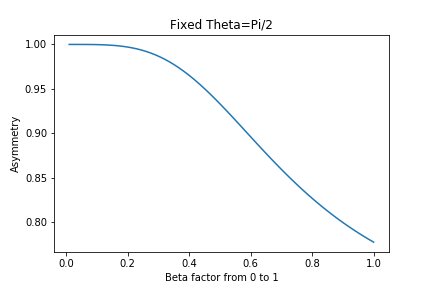
\includegraphics[scale=0.5]{Asymmetry_vs_Beta.png}
\centering
\caption{Asymmetry as a function of $\beta$ at a fixed $\theta=\pi/2$, where the asymmetry is maximal.}
\label{fig:AsymmetryVsBeta}
\end{figure}

In our experiment, electrons with mass of $0.511 \MeV$ are emitted Yttrium-90 with a maximum energy of $2.28 \MeV$, and an average energy of 0.93 \MeV. To the maximum energy corresponds a $\gamma=4.46$ and a $\beta=0.95$. To the average energy corresponds a $\gamma=1.83$ and a $\beta=0.84$. So we also plot in Figure~\ref{fig:AsymmetryVsTheta} the asymmetry as a function of the angle $\theta$ in the particular cases when $\beta=0.84$ and $\beta=0.95$. At both values the asymmetry is close to minimal, which is obtained for $\beta=1.0$. The plots also confirm that the asymmetry is maximal at $\theta=\pi/2$. 

\begin{figure}[H]
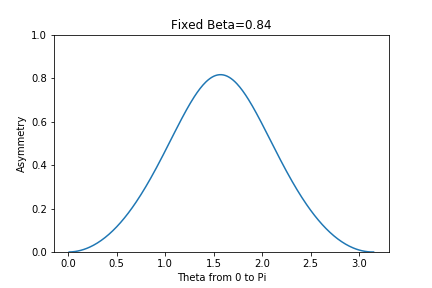
\includegraphics[scale=0.5]{Asymmetry_vs_Theta_84.png}
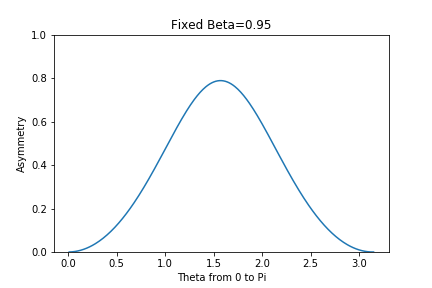
\includegraphics[scale=0.5]{Asymmetry_vs_Theta_95.png}
\centering
\caption{Asymmetry as a function of $\theta$ at a fixed $\beta=0.84$ and $\beta=0.95$, representative for our experiment.}
\label{fig:AsymmetryVsTheta}
\end{figure}

\subsection{Asymmetry and experimental observables}
\label{asym_measurement}

In this experiment we are measuring the asymmetry by counting the number of electrons arriving to the detectors. Thus, finding the relation between the asymmetry of cross sections and the count rate of the detectors is crucial.\\

Some of the electrons detected have no correlation between their polarisations. Therefore we have to define the cross section of unpolarised electrons, $\sigma_0 = 1/2 (\sigma_{\leftleftarrows} + \sigma_{\rightleftarrows})$.\\

Denoting $P_{\rm s}$ as the longitudinal polarisation of the incoming electrons emitted by the source and $P_{\rm t}$ the longitudinal polarisation of the electrons in the target, we can define the count rate for the electrons with parallel polarisation ($C_{\leftleftarrows}$) and antiparallel polarisation ($C_{\rightleftarrows}$) as

\begin{equation}\label{28}
C_{\leftleftarrows} \approxeq P_{\rm s} \cdot  P_{\rm t}  \cdot  \sigma_{\leftleftarrows} + (1-P_{\rm s}  \cdot P_{\rm t}) \cdot  \sigma_0,
\end{equation}
\begin{equation}
C_{\rightleftarrows} \approxeq P_{\rm s}  \cdot  P_{\rm t}  \cdot  \sigma_{\rightleftarrows} + (1-P_{\rm s}  \cdot P_{\rm t}) \cdot \sigma_0.
\end{equation}

Using the previous relations we can define $\epsilon$ as the asymmetry of the count rate for the two cases with parallel and antiparallel polarisations:

\begin{equation}\label{30}
\epsilon=\frac{C_{\rightleftarrows}-C_{\leftleftarrows}}{C_{\rightleftarrows}+C_{\leftleftarrows}} \approxeq P_{\rm s}  \cdot  P_{\rm t}  \cdot \frac{\sigma_{\rightleftarrows}-\sigma_{\leftleftarrows}}{\sigma_{\rightleftarrows}+\sigma_{\leftleftarrows}}= P_{\rm s} \cdot P_{\rm t} \cdot A(\theta,\beta).
\end{equation}

In this way we succeed in relating the asymmetry of the cross section ($A(\theta,\beta)$) with experimental observables: the asymmetry in the counting rate ($\epsilon$), polarisation of the source electron ($P_{\rm s}$), and the polarisation of the target electron ($P_{\rm t}$).

\section{Kinematics}

Cross sections are easy to compute in the centre-of-mass (c.o.m or com) frame, while the experiments are easy to be expressed in the laboratory (lab) frame. In this section we relate the two frames. This will also help us show that the positions of the detectors are chosen so that the asymmetry is maximised. \\

The interaction we use in our experiment,  $e^- + e^- \rightarrow e^- + e^-$, is an elastic collision (at all energies), as illustrated in Figure~\ref{fig:lab} for both the lab frame (left) and the center-of-mass frame (right).

\begin{figure}[H]
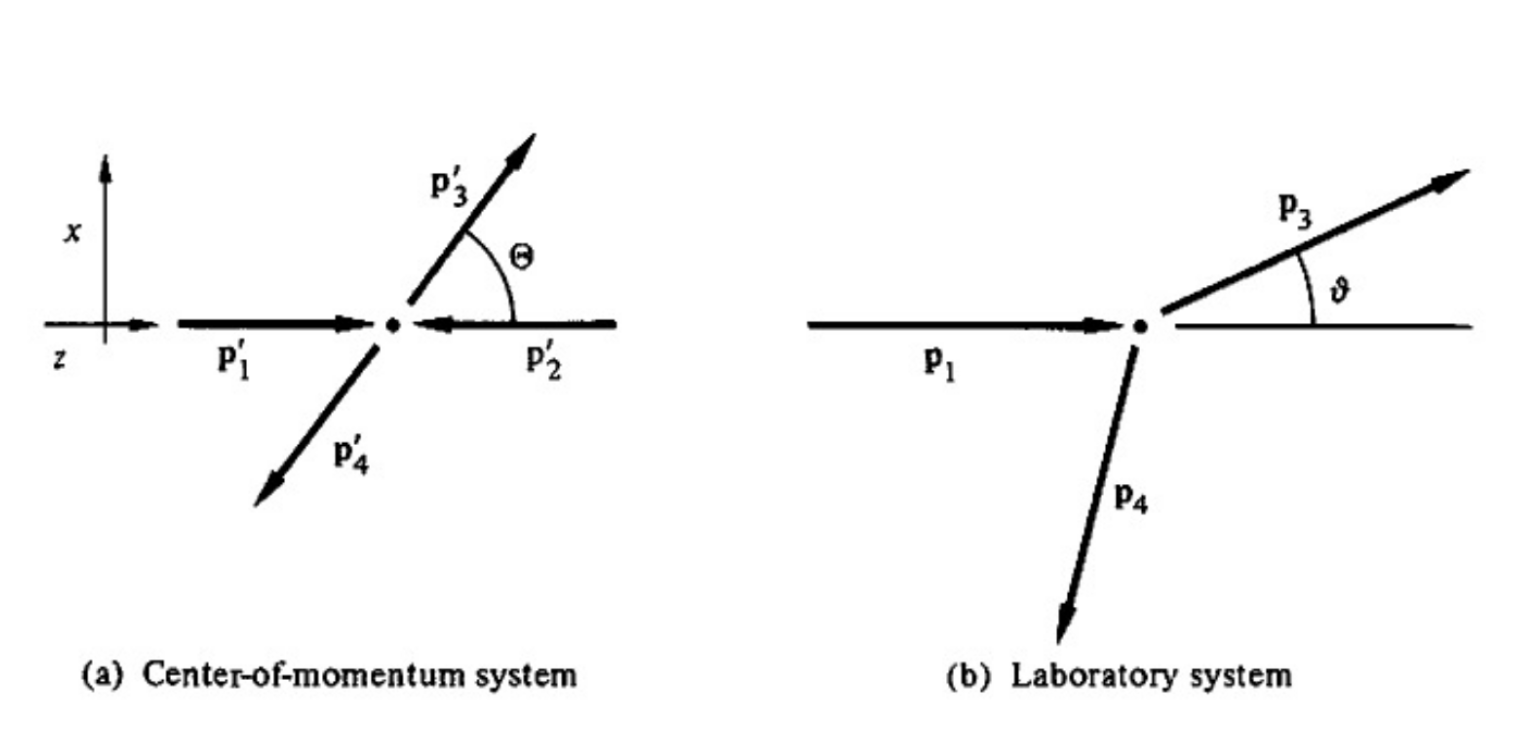
\includegraphics[scale=0.5]{ScatteringTwoFrames.png}
\centering
\caption{Comparison between scattering in the c.o.m (left) and lab (right) eference frames.}
\label{fig:lab}
\end{figure}

With the initial quadri-vectors (4-vectors) we can define

\begin{equation}
    P^{\mu}_{\rm lab,1} = (E_{\rm lab,1},p_{\rm lab,1},0,0)
\end{equation}

\begin{equation}
    P^{\mu}_{\rm lab,2} = (m_e,0,0,0)
\end{equation}

\begin{equation}
    P^{\mu}_{\rm com,1} = (E_{\rm com,1},p_{\rm com,1},0,0)
\end{equation}

\begin{equation}
    P^{\mu}_{\rm com,2} = (E_{\rm com,2},-p_{\rm com,1},0,0)
\end{equation}

After the collision, using energy conservation and the fact that the norm of the 4-vectors are equals, $P^{\mu}_{\rm com,3} = (E_{\rm com,1},p_{\rm com,1}\cos{\theta_{\rm com}},p_{\rm com,1}\sin{\theta_{\rm com}})$, we can perform a Lorentz transformation to obtain the 4-vector in the lab frame as

\begin{equation}
P^{\mu}_{\rm lab,3} = \begin{pmatrix}
\gamma & \gamma\beta & 0 & 0 \\
\gamma\beta & \gamma & 0 & 0\\
0 & 0 & 1 & 0\\
0 & 0 & 0 & 1
\end{pmatrix};
P^{\mu}_{\rm com,3} = \begin{pmatrix}
\gamma[E_{\rm com,1}+\beta p_{\rm com,1}\cos{\theta_{\rm com}}]\\
\gamma[\beta E_{\rm com,1}+ p_{\rm com,1}\cos{\theta_{\rm com}}]\\
p_{\rm com,1}\sin{\theta_{\rm com}}]\\
0
\end{pmatrix}.
\end{equation}

By looking at Figure~\ref{fig:lab} we can find a relation for the angle in the lab frame

\begin{equation}\label{eq:2}
    \tan{\theta_{\rm lab}} = \frac{P^y_{\rm lab,3}}{P^x_{\rm lab,3}} = \frac{\sin{\theta_{\rm com}}}{\gamma(\cos{\theta_{\rm com}}+\frac{\beta E_{\rm com,1}}{p_{\rm com,1}})}.
\end{equation}

For solving this equation first of all, we will focus on the energy and momentum of the c.o.m term, which by using a Lorentz transformation we can express as

\begin{equation}\label{eq:3}
    \frac{\beta E_{\rm com,1}}{p_{\rm com,1}} = \frac{\beta (E_{\rm lab,1}-\beta p_{\rm lab,1})}{p_{\rm lab,1}-\beta E_{\rm lab,1}}.
\end{equation}

In the centre-of-mass the speed of the particle can be expressed as $v_{\rm com,1} = \frac{p_{\rm com,1}}{E_{\rm com,1}}$, where $v_{\rm com,1} = \beta_{\rm com,1}$, since the speed of light is considered to be one ($c=1$). Using this relation we can set the equivalence

\begin{equation}\label{eq:4}
    \frac{\beta E_{\rm com,1}}{p_{\rm com,1}} = \frac{\beta}{\beta_{\rm com,1}}.
\end{equation}

By imposing that $P^x_{\rm lab,1}=-P^x_{\rm lab,2}$, we are lead to the expression
\begin{equation}\label{eq:1}
    \beta = \frac{p_{\rm lab,1}}{E_{\rm lab,1}+m_e}.
\end{equation}

By also using the relation $E_{\rm lab,1}=E_{\rm kinetic}+m_e$ we find 

\begin{equation}\label{eq:5}
    \frac{\beta}{\beta_{\rm com,1}} = 1.
\end{equation}

From Equation \ref{eq:1} we can rewrite the Lorentz factor as
\begin{equation}\label{eq:6}
    \gamma = \frac{1}{\sqrt{1-\beta^2}}= \frac{E_{\rm kinetic}+m_e}{\sqrt{4m_e^2 + 2 E_{\rm kinetic}m_e}}.
\end{equation}

By using the Equations \ref{eq:4}, \ref{eq:5} and \ref{eq:6}, and the fact that $\theta_{\rm com} = \pi/2$ to maximise the asymmetry, as explained in Section~\ref{asym}, we determine the angle in the laboratory frame as

\begin{equation}
    \tan{\theta_{\rm lab}}= \frac{1}{\gamma}\frac{\sin{(\pi/2)}}{\cos{(\pi/2)}+1} = \frac{1}{\gamma} = \frac{\sqrt{4m_e^2 + 2 E_{\rm kinetic}m_e}}{E_{\rm kinetic}+2m_e}.
\end{equation}

Using energy conservation, the total energy of the exiting electron has half of the energy of incoming energy,  or $E_{\rm outgoing} = E/2$. We plot that in Figure \ref{fig:theta}, where we can see the scattering angle in the lab frame as a function of the incident particle at a fixed angle in the centre-of-mass.\\

\begin{figure}[h]
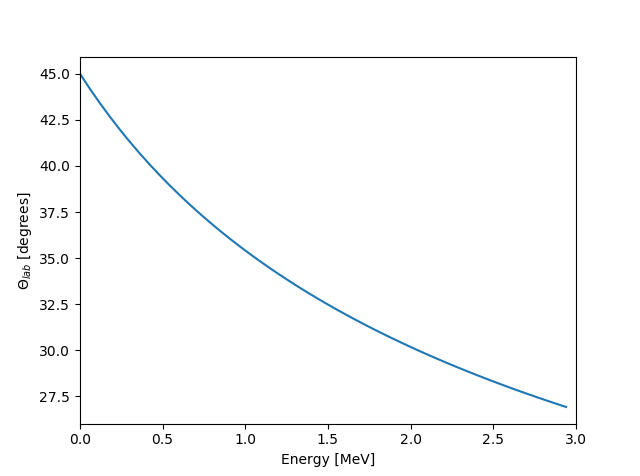
\includegraphics[scale=0.5]{theta.png}
\centering
\caption{Diffusion angle in the lab as a function of the incident kinetic energy.}
\label{fig:theta}
\end{figure}

Since the Yttrium-90 source is disintegrated with an average energy of 0.927 \MeV~and a maximal energy of 2.28 \MeV, as illustrated in Figure~\ref{fig:Sr90}, we can say that the electrons will be scattered with angles around 35. Thus, we fixed the detectors at $35 \pm 11$ degrees, as illustrated in Figure~\ref{fig:TwoDetectors}. In this way, we maximise the possibilities of detecting most of the events. \\

\begin{figure}[h]
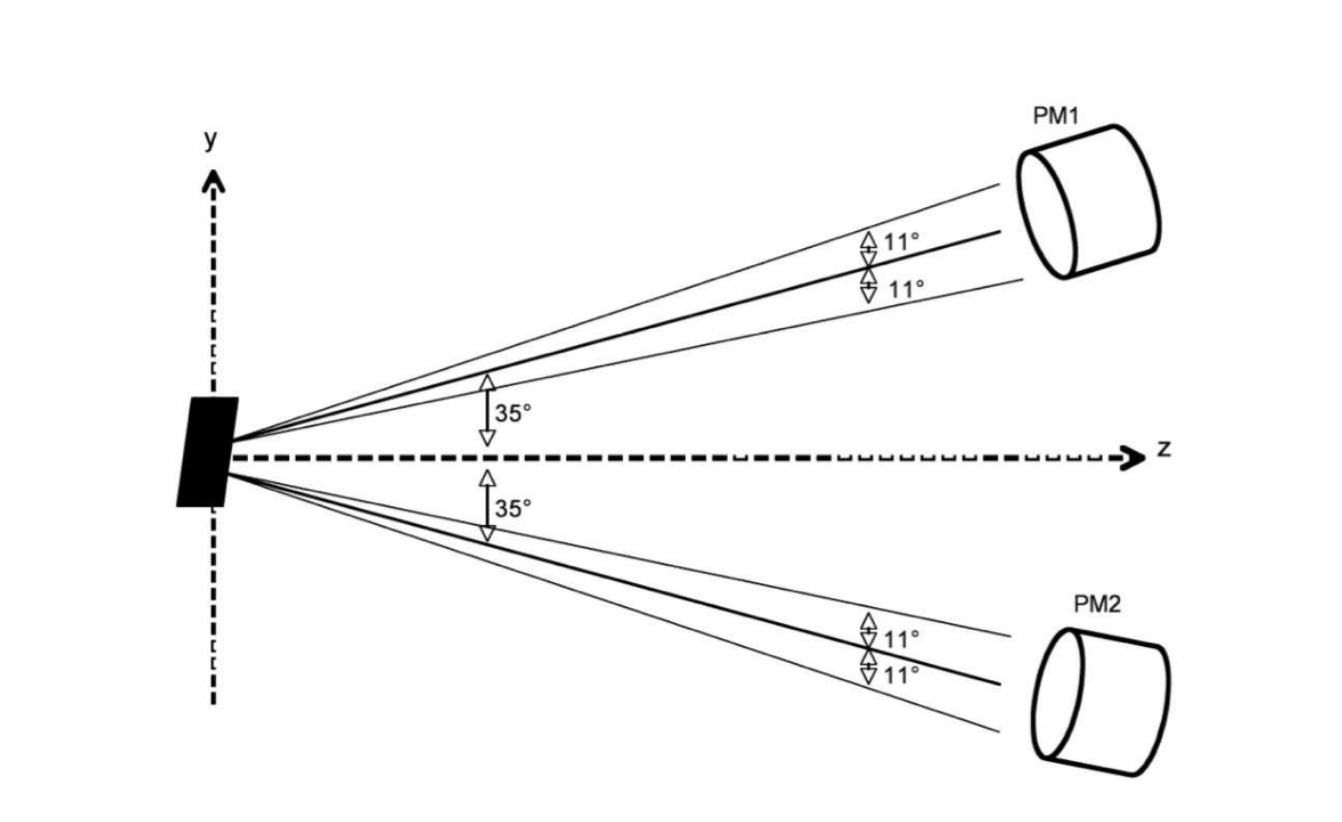
\includegraphics[scale=0.5]{TwoDetectors.png}
\centering
\caption{The two detectors are placed symmetrically around the z-axis at 35 degrees each. The detectors are circular, each radius being seen with an angle of 11 degrees.}
\label{fig:TwoDetectors}
\end{figure}

\chapter{Experimental setup}
\label{chapter:ExperimentalSetup}

\section{Setup}
\begin{figure}[h]
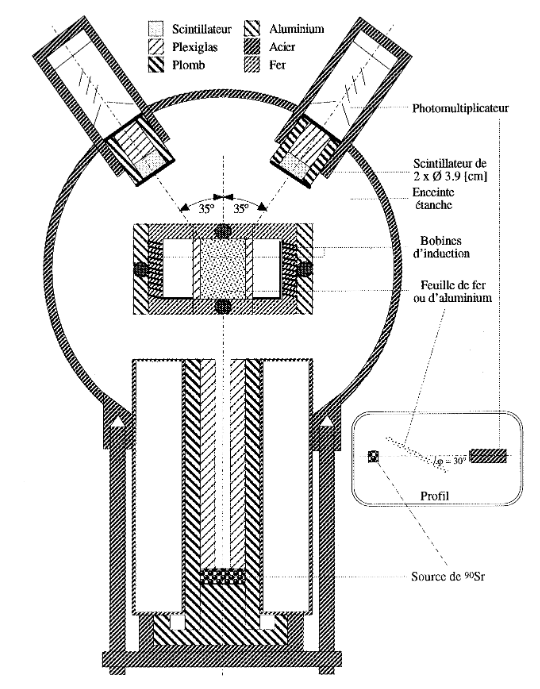
\includegraphics[scale=0.5]{setup.png}
\centering
\caption{Schema of the experimental setup.}
\label{fig:setup}
\end{figure}

Figure \ref{fig:setup} illustrates an overview of the experimental setup. For this experiment we are using as a $\beta$ emitter a Strontium-90 source, which is located in the lower part of the schema. It is surrounded by lead to avoid the radiation goes outside. The source is facing an enclosure of around 35 cm of diameter that can be closed with a lid, which is made of the same material as the enclosure, namely steel.\\

Oriented at an angle of $35 \pm 11$ degrees, as mentioned before, in the right and left sides of the target there are two plastic scintillators, each one coupled to a light guide and a photomultiplier. The electrons coming from the Moller scattering off the target lose energy when traversing the scintillator, which leads to an excitation of its molecules. The excited molecules from the scintillator tends to find their minimum energy by losing this excess energy in the form of emitted photons, which are guided through the photomultipliers by the guide lights.\\

An image of the physical setup is illustrated in Figure~\ref{fig:setupexp}.

\begin{figure}[h]
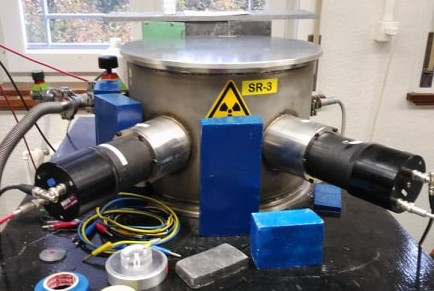
\includegraphics[scale=0.8]{experimentalsetup.jpg}
\centering
\caption{Actual image of the experimental setup.}
\label{fig:setupexp}
\end{figure}

In the middle of the enclosure there is the support where the target is fixed, namely an aluminium or iron target, as well as the induction coils, as seen in Figure \ref{fig:cible}.

\begin{figure}[H]
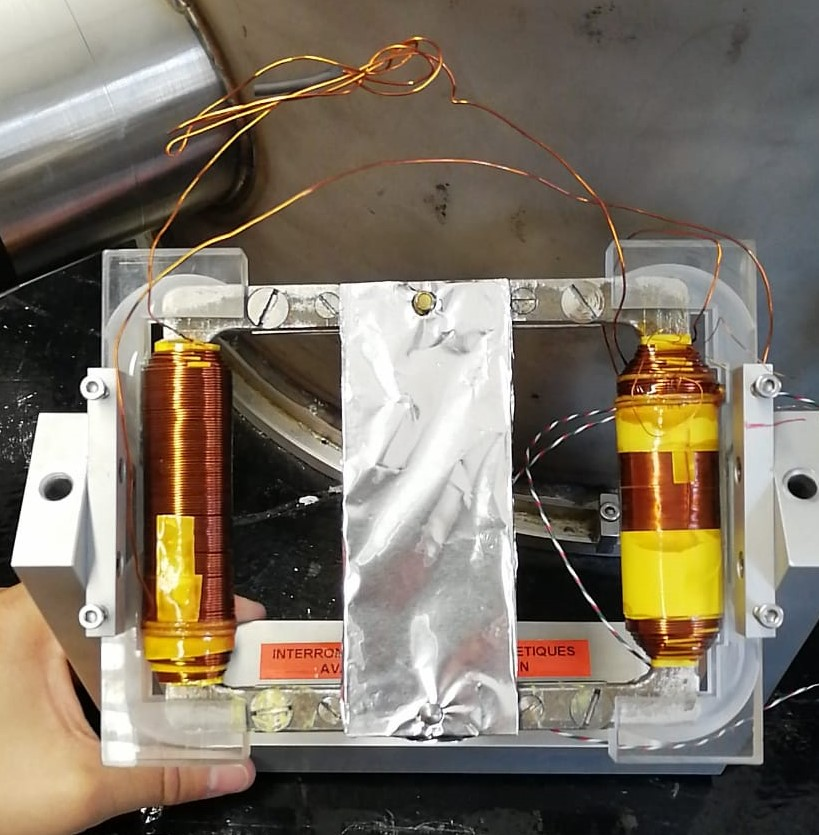
\includegraphics[scale=0.3]{cible.jpeg}
\centering
\caption{Actual image of the target.}
\label{fig:cible}
\end{figure}

The incident electrons coming from the source are interacting with the electrons in the target via Moller scattering. As said in the previous section, the electrons coming from the source have a longitudinal polarisation. Thanks to the coils, we can control the magnetic field applied to the target. Therefore we can control the polarisation of the electrons in the target, making them either parallel or antiparallel relative to the ones coming from the source. An iron foil is used as a target given its ferromagnetic properties. We can then change the orientation of all the spins in the target, using a low magnetic field. \\

All the components are placed in vacuum, at approximately 1.8 mbar, in order to minimise the electron energy lost and multiple scattering with air particles.

\section{Radioactive Source}

The source used in this experiment is Strontium-90 ($\prescript{90}{38}{\mathbf{Sr}}$). It disintegrates into Yttrium-90 ($\prescript{90}{39}{\mathbf{Y}}$) via the beta decay ($\beta$-decay), which produces one electron and one electron antineutrino, with a half-life of 28.79 years, as illustrated in left side of Figure~\ref{fig:Sr90}. This is the only channel of disintegration and is described by

 \begin{equation}
     \prescript{90}{38}{\mathbf{Sr}} \rightarrow \prescript{90}{39}{\mathbf{Y}} + e^- +\bar{\nu}_e.
 \end{equation}
 
In turn, Yttrium-90 decays with a half-time of 64 hours via the $\beta$-decay into Zirconium-90 ($\prescript{90}{40}{\mathbf{Zr}}$), , as illustrated in left side of Figure~\ref{fig:Sr90}, and creating again, another electron and another electron antineutrino, as given by
 
\begin{equation}
     \prescript{90}{39}{\mathbf{Y}} \rightarrow \prescript{90}{40}{\mathbf{Zr}} + e^- +\bar{\nu}_e .
 \end{equation}

The energy of the electrons released during the first disintegration has a maximum of  0.546 \MeV, and an average value of 0.196 \MeV. For the second disintegration the maximum energy released by the electron is 2.28 \MeV, with the average value of 0.927 \MeV. These values are illustrated in the right side of Figure~\ref{fig:Sr90}. As discussed before, the electrons measured in this experiment are the ones coming from the second disintegration. This fact will be an automatic consequence due to the energy range used to treat the data, as described in the following chapters.

\begin{figure}[H]
\includegraphics[scale=0.4]{Sr90.jpg}
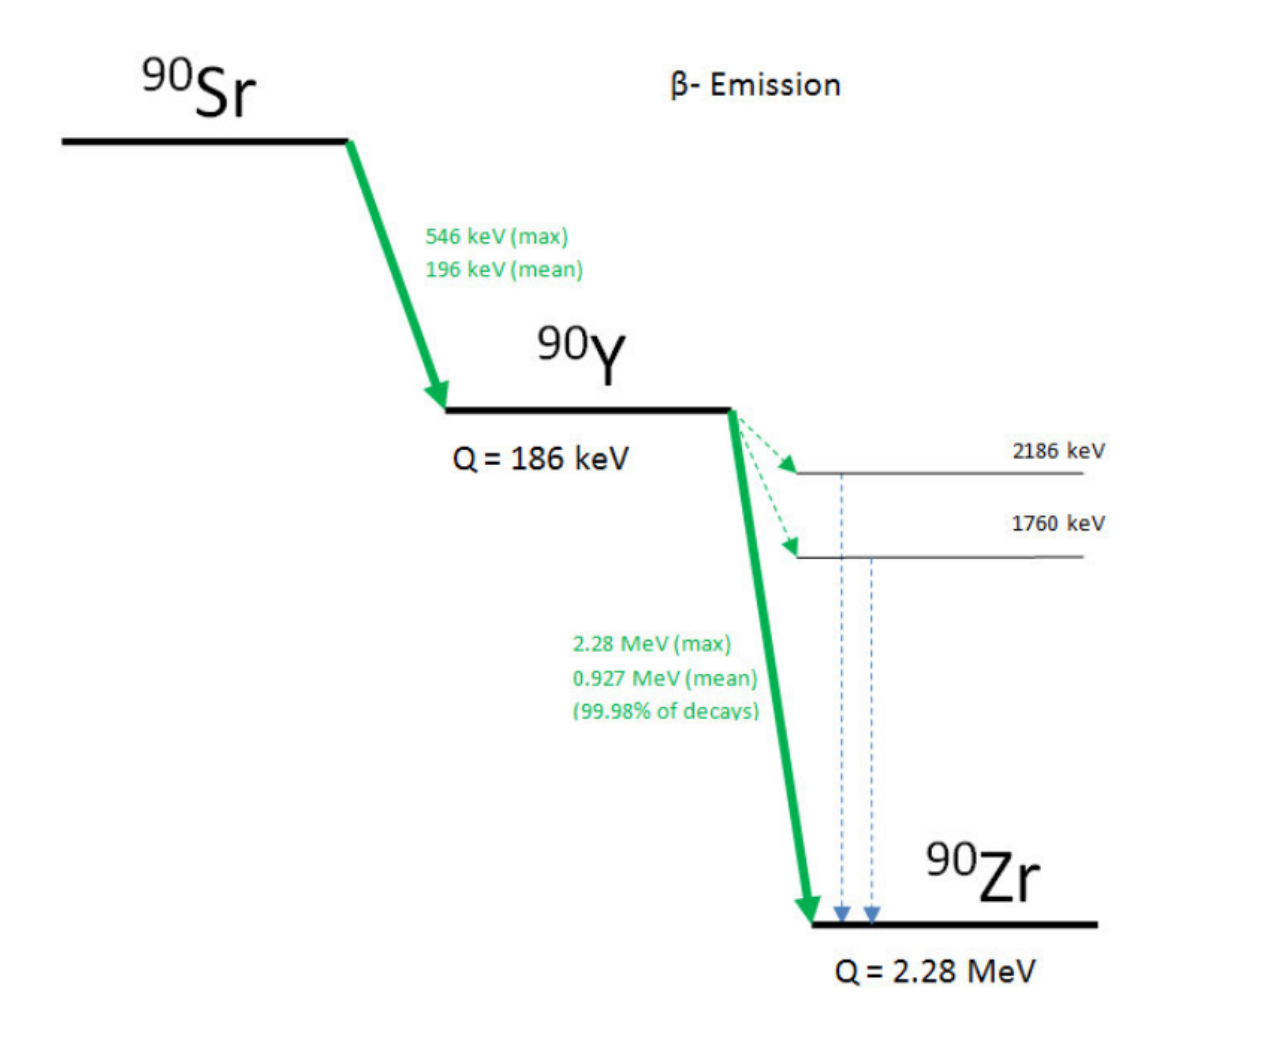
\includegraphics[scale=0.3]{Sr90_2.png}
\centering
\caption{Strontium-90 decay diagrams. The left one presents also life-times. The right one presents also average energies of emitted electrons. For Strontium-90, the maximum (average) value for the energy of the electron is 0.546 \MeV (0.196 \MeV). For Yttrium-90, the maximum (average) value for the energy of the electron is 2.28 \MeV (0.927 \MeV).}
\label{fig:Sr90}
\end{figure}

\section{Photomultiplier tube}

A photomultiplier tube (PMT) is a detector sensible to light, widely use in high energy physics. As illustrated in Figure \ref{fig:PMT}, a PMT consists of a photocathode, a chain of dynodes and an anode. The photocathode is negatively charged and recoated with a material capable of releasing an electron as soon as a photon arrives, due to the photoelectric effect. A dynode is an electrode in a vacuum tube that serves as an electron multiplier through secondary emission.

\begin{figure}[H]
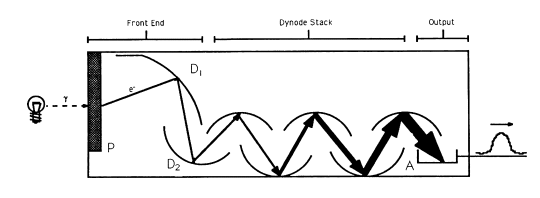
\includegraphics[scale=0.5]{PMT.png}
\centering
\caption{Schematic of a Photomultiplier tube.}
\label{fig:PMT}
\end{figure}

As said before, the electrons emitted from the cathode are accelerated toward the first dynode. Each accelerated photoelectron that strikes the dynode surface frees several electrons from the surface. These electrons are then accelerated toward the second dynode, held more positive than the first dynode. Each electron that strikes the surface of the second dynode produces several more electrons, which are then accelerated toward the third dynode, and so on. Thus a multiplication of the signal is produced.\\

The photomultipliers tubes used in this experiment are manufactured by Hamamatsu. They have with a diameter of 5.1cm and contain a photo-sensible surface of a diameter of 4.6 cm. The gain, or ratio between the secondary electrons between two dynodes, increases exponentially with the applied voltage.
In order to chose the optimised value for the tension applied to the PMT, a calibration is needed, as discussed in Chapter~\ref{chapter:Calibration}.

\section{Electronics}

This amplified signal arrives to the electronics. Its schematic treatment there is illustrated in Figure~\ref{fig:electronicsSchema}, while the actual image of the electronics of the experiment is presented in Figure~\ref{fig:electronicsActual}.

\begin{figure}[H]
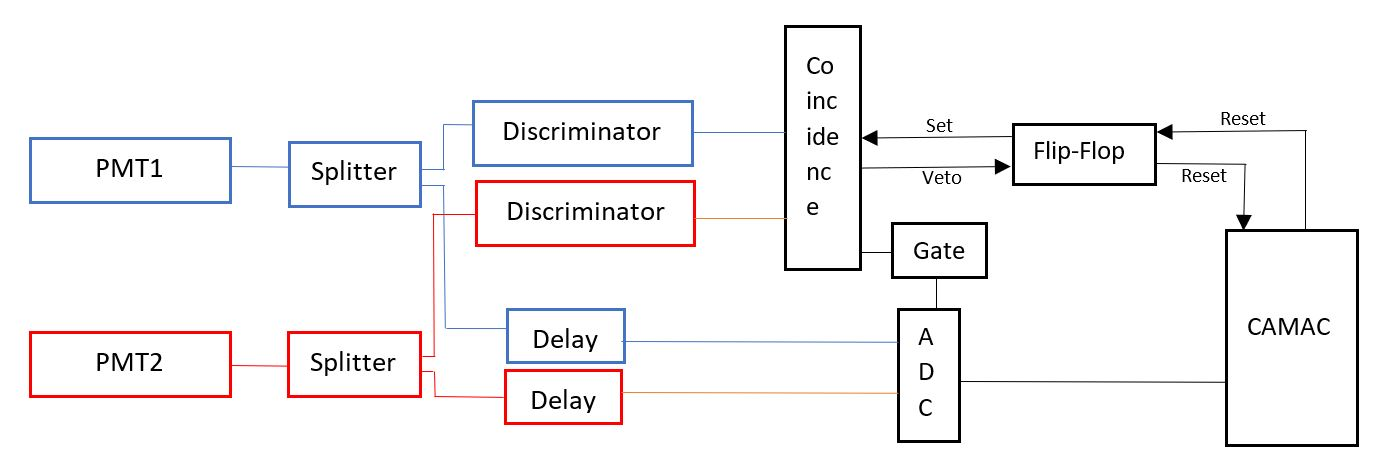
\includegraphics[scale=0.5]{electronics.JPG}
\centering
\caption{Schema of the electronics}
\label{fig:electronicsSchema}
\end{figure}

The two signals coming from the two PMTs each arrive to a splitter, which divides each signal in two outputs. \\

One of the two outputs for each of the signals of PMT1 and PMT2 is connected to a discriminator. The discriminator converts the analog signal into a digital (ADC) one, with a fixed width (30 ns) and threshold (50 mV), which only allows certain values of the signal. The outputs of both discriminators are input to the coincidence device, which works as a trigger.  It is during this time that the signals coming from the second splitter must also arrive, in order for the trigger to be produced. When a coincidence happens and the event has been read, the PC, through the CAMAC controller, resets the system via the flip-flop device, avoids the trigger to overlap within different events.\\

The other output from the splitters for each of the two signals of PMT1 and PMT2 is connected to a delay line, that represents the window in which the ADC module is acquiring data coming from the PMTs after passing through a delay. This delay is needed to ensure that the signals coming from the PMT arrives to the ADC in the acquiring window set by the gate. This process avoids the overlap between different events. Thus there is a dead time, during which the system is not acquiring new data. During this time, the ADC is converting the signal into binary data. The CAMAC will read this data and send it to the computer where it will be stored. Once the data is read, the CAMAC resets the flip-flop and new data can be acquired.

\begin{figure}[H]
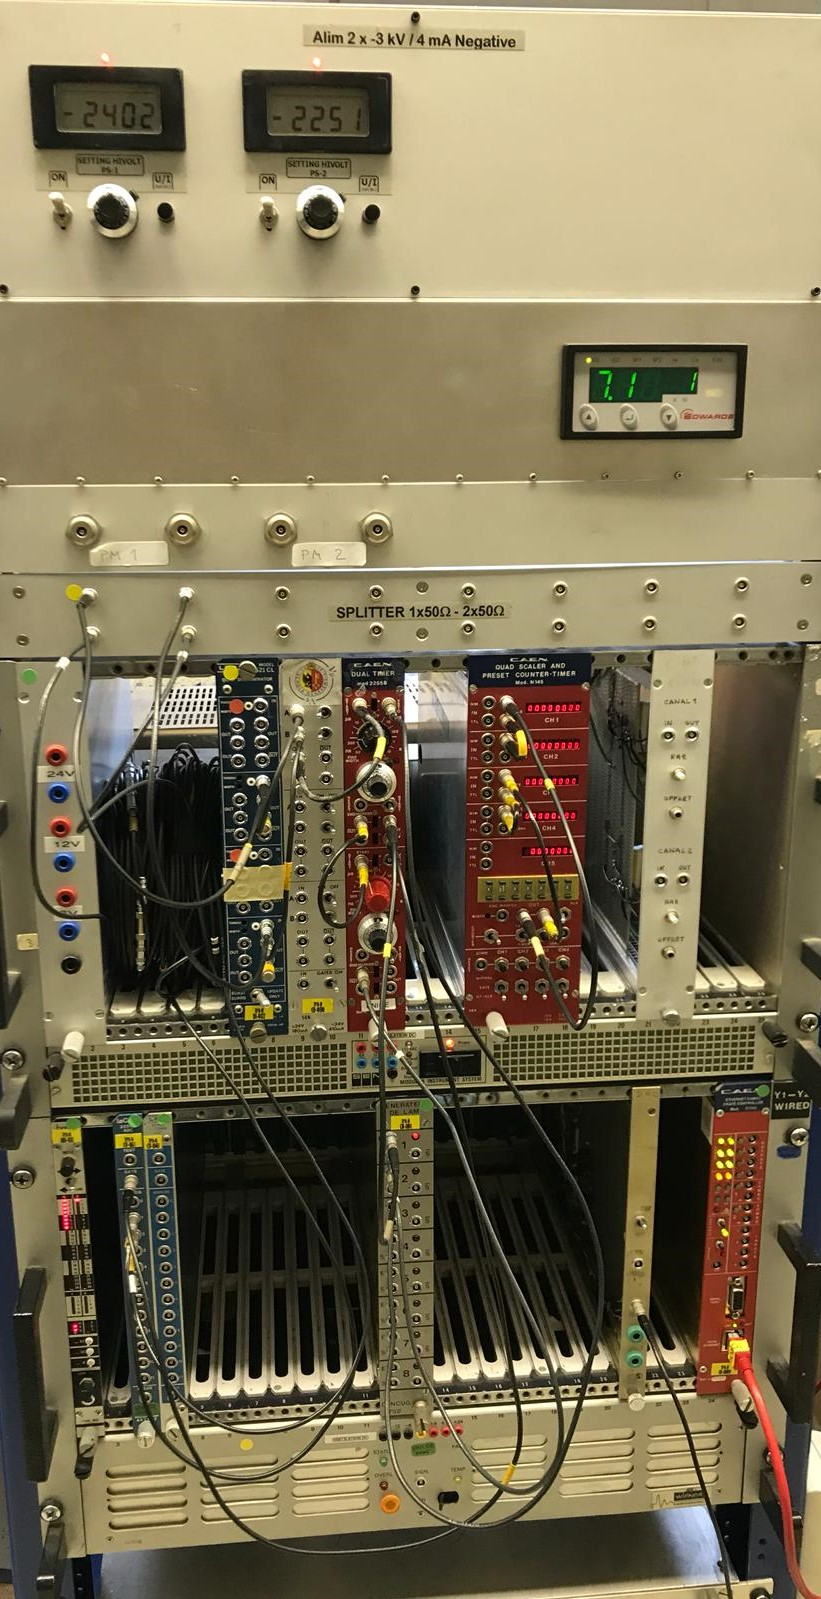
\includegraphics[scale=0.3]{electronics.jpeg}
\centering
\caption{Actual image of the electronics of the experiment.}
\label{fig:electronicsActual}
\end{figure}

\chapter{Calibration and measurements}
\label{chapter:Calibration}

The formal definition of calibration by the Bureau International des Pois et Mesures (BIPM) is ``an operation that, under specified conditions, in a first step establishes a relation between the quantity values with measurement uncertainties provided by measurement standards and corresponding indications with associated measurement uncertainties and, in a second step, uses this information to establish a relation for obtaining a measurement result from an indication.'' Therefore the calibration of the PMTs used in this experiment is crucial.

\section{Calibration}

We need to determine the optimal working regime of the PMTs in our experiment. We need to focus mainly in the linearity, the resolution, the coincidence and the energy. \\

For doing this calibration we make two sets of measurements: with no signal to measure the background, and adding a signal from $\prescript{207}{}{Bi}$. In each measurement we plot the histogram distribution (Count) for various voltages measured by the PMT (converted to digital value as an ADC value), each corresponding to one energy of an incoming photon. We repeat these experiments for various high voltages at which the PMT operate, to choose the best operating point. \\

The background distributions of counts vs ADC when there is no source are presented in Figure~\ref{fig:background}, for PMT1 and PMT2, working at high voltages of 2200 V and 2250 V, respectively. The high voltages are optimised for the signal, as described later in the section. As expected, both distributions looks similar, with a very narrow and tall peak around 0 ADC and falling very abruptly. There is basically no background at high ADC larger than 1000. The peak is fit with a Gaussian distribution. The average value $\mu_{\rm background}$ is actually not zero, although very close to zero, and it corresponds to zero energy of the incoming photon. This is also called the pedestal of the PMT. For PMT1 and PM2 the ADC for zero energy or pedestal is 45 and 30, respectively.\\

\begin{figure}[H]
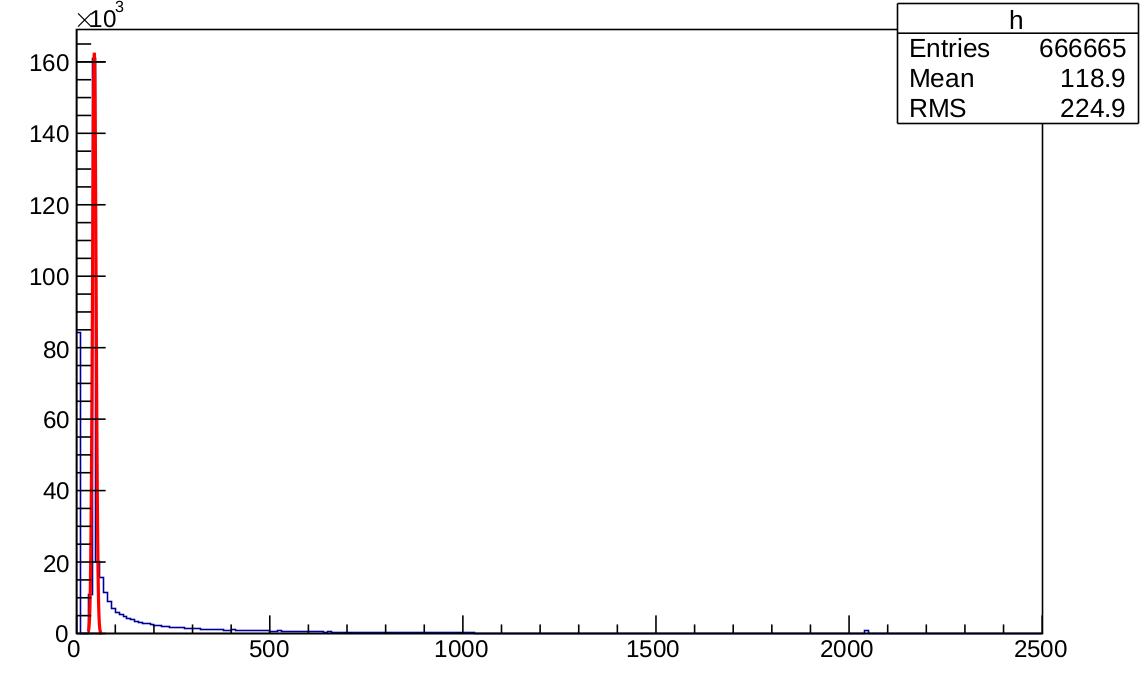
\includegraphics[scale=0.20]{background1.png}
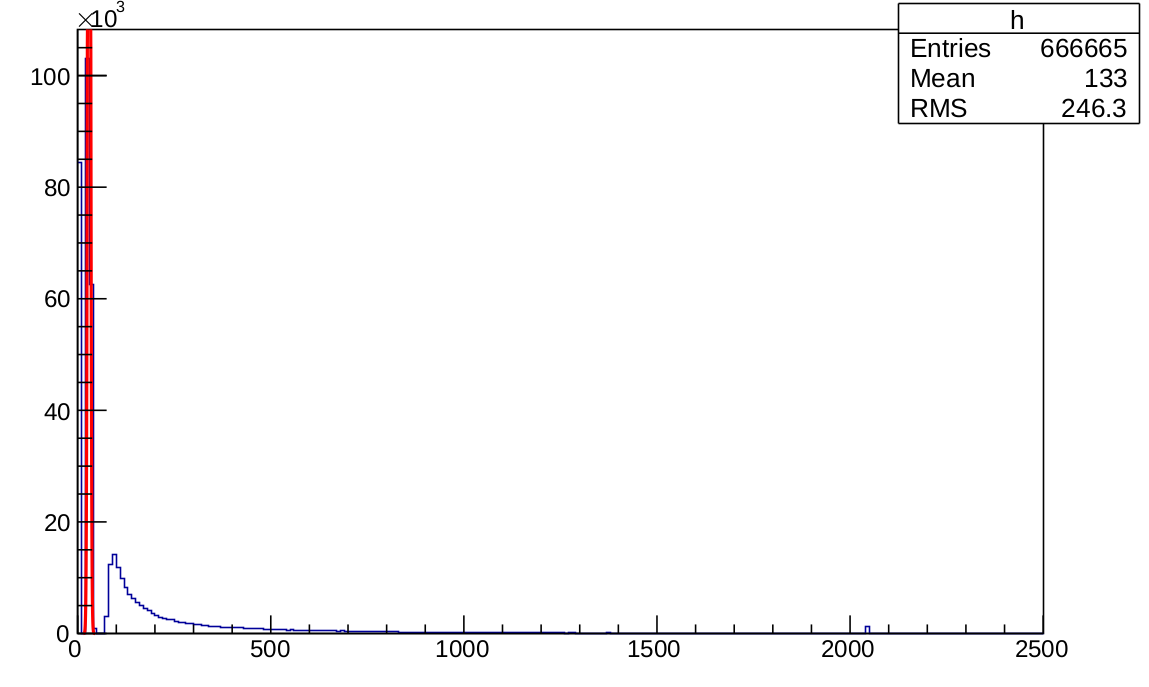
\includegraphics[scale=0.20]{background2.png}
\centering
\caption{Background distribution of counts vs ADC, when there is no source, for PMT1 (left) and PMT2 (right), operating at high voltages 2200 V and 2250 V, respectively.}
\label{fig:background}
\end{figure}


The signal distribution of counts vs ADC when a source of $\prescript{207}{}{Bi}$ is presented as an example in Figure~\ref{fig:spectrum} for PMT2, in the case when the high voltage is 2100 V. 

\begin{figure}[H]
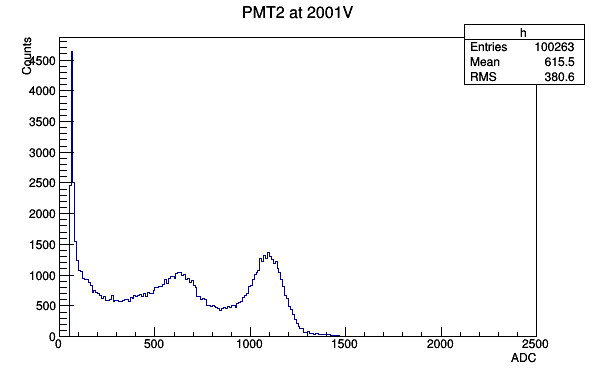
\includegraphics[scale=0.7]{spectrum.png}
\centering
\caption{Signal distribution for the source $\prescript{207}{}{Bi}$ for PMT2, operating at the high voltage of 2100 V.}
\label{fig:spectrum}
\end{figure}

We observe three peaks in the distribution. The one close to zero ADC is due to background, present even when there is no signal source, evaluated in the discussion above. The second and the third peaks are due to the Bismuth signal. We fit the third peak (the second peak of Bismuth) with a Gaussian and extract its mean $\mu$ and standard deviation $\sigma$ for various high voltages for the PMT operation. \\ 

The variation of the mean ADC for the second Bismuth peak vs the high voltage is shown in Figure~\ref{fig:mean}. We observe there is a linear relationship for both PMTs: the larger the high voltage, the higher the Gaussian mean of the ADC counts for the same physical process. 

\begin{figure}[H]
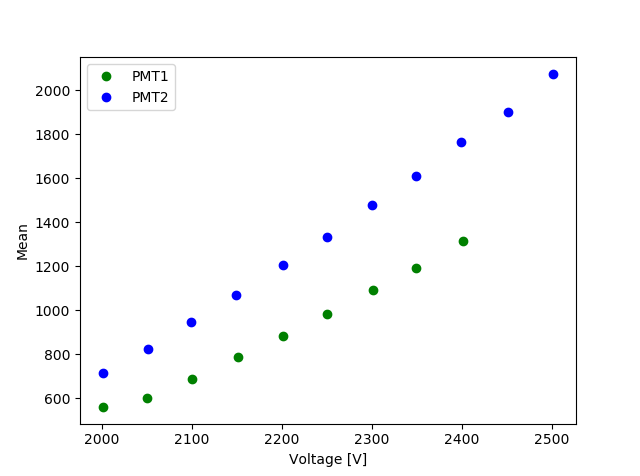
\includegraphics[scale=0.6]{mean.png}
\centering
\caption{Mean ADC for the second signal peak as a function of the high voltage for both PMTs.}
\label{fig:mean}
\end{figure}

Since for both PMTs we are in the linearity region, we can choose any desired high voltage without restriction between 2000 V and 2500 V. To choose one operating high voltage for each PMT, the PMT resolution is taken into account.  The resolution is given by

\begin{equation}
    R = \frac{\sigma}{\Delta\mu} =  \frac{\sigma}{\mu - \mu_{\rm background}},
\end{equation}

where $\sigma$ is the standard deviation for the signal, $\mu$ is the mean for the signal and  $\mu - \mu_{\rm background}$ is the mean for the background evaluated above. Figure~\ref{fig:res} presents the resolution as a function of the high voltage for both PMTs.

\begin{figure}[H]
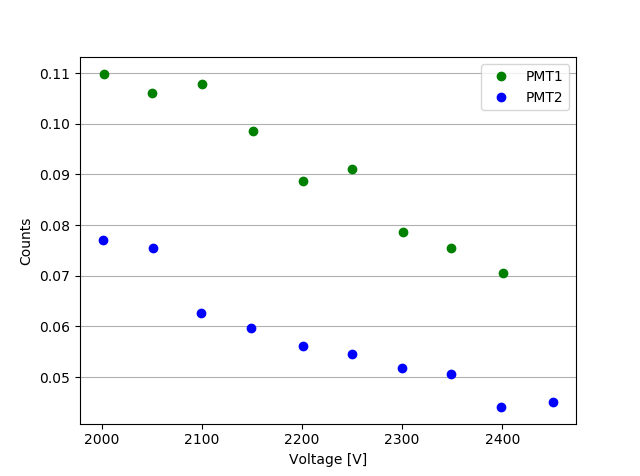
\includegraphics[scale=0.6]{Resolution.png}
\centering
\caption{Resolution as a function of the high voltage for both PMTs.}
\label{fig:res}
\end{figure}

By analysing this plot we can choose the best working voltage for each PMT. The tension is set to be 2200 V for the PMT1 and 2250 V for PMT2.\\

The rate of the coincidences as a function of the high voltage for each PMT, while keeping the other fixed at 2350 V, is shown in Figure~\ref{fig:coincidence} . At 2200 V in the PMT1 and 2250 V in PMT2 the rate blows up because the high voltage in the PMTs multiplies the number of electrons created (gain). Therefore it is found found that the optimal voltage is well outside the region of the plateau. In order to find a stable region around the set voltages it is necessary to change the discriminator parameters, the threshold and the width.

\begin{figure}[H]
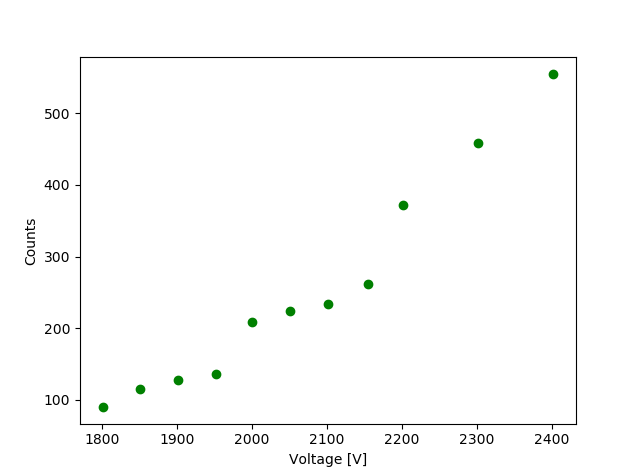
\includegraphics[scale=0.5]{CoincidencePMT1.png}
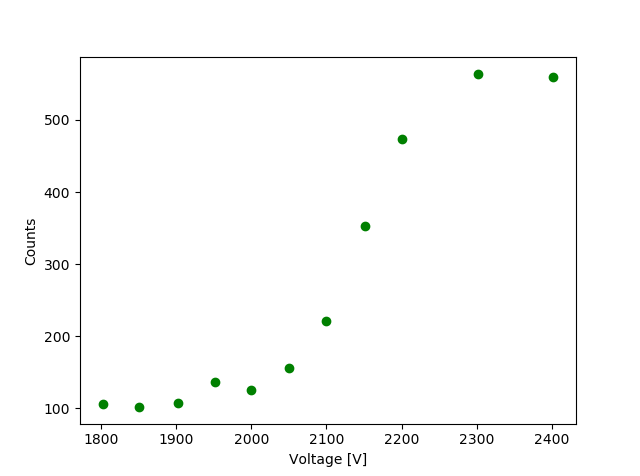
\includegraphics[scale=0.5]{CoincidencePMT2.png}
\centering
\caption{Coincidences vs high voltage in PMT1 with PMT2 fixed at 2350 V (left), and in PMT2 with PMT1 fixed at 2350 V (right).}
\label{fig:coincidence}
\end{figure}

In order to set the voltage within the plateau, the threshold of the discriminator has been changed to 150 mV.\\

By studying the coincidences as a function of the width of the discriminator we can conclude that when the width is too small no coincidences are observed. By increasing the width, we reach the plateau and for even higher values too many coincidences are counted and the rate of the coincidences quickly increase similarly for what happened with the coincidences as a function of the voltage. As a result, the width has been chosen to be 30 ns, in order to avoid accidental coincidences.\\

With the high voltage already set, the last step is to find the equivalence between the ADC channel and energy of the incoming photon. The electronics output is in ADC. We need to interpret it in energy, so we need to convert ADC into energy. We need to make two assumptions. First of all, we have to assume a linear dependence between the ADC channel and the detector response (energy). The second one regards value of the ADC, when there is no signal of incoming particle, so the ADC value corresponding to the zero energy, also called pedestal, evaluated above in Figure~\ref{fig:background}.\\

In Figure~\ref{fig:spectrum}, as mentioned before, we discuss the spectrum of a $\prescript{207}{}{Bi}$ source. We know the energy of the second Bismuth peak to be 1.06 \MeV, so we can establish a linear relation between this energy and the ADC channel for each PMT. For doing that we fitted the second Bismuth peak for the PMT1 at an operating high voltage of 2200 V (obtaining the mean value of 885 ADC) and for the PMT2 at an operating high voltage of 2250 V, obtaining the mean value of 1334 ADC, as illustrated in Figure \ref{fig:pmt_fits}.

\begin{figure}[H]
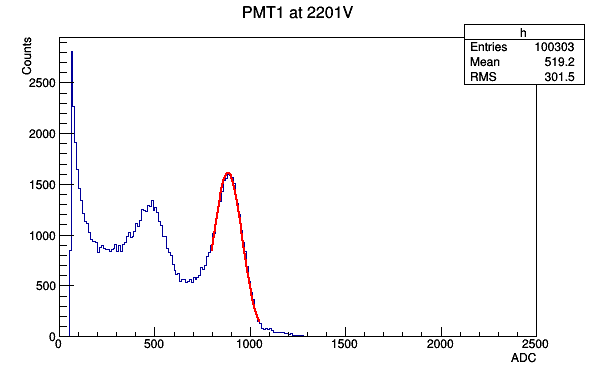
\includegraphics[scale=0.39]{PMT1_2201V.png}
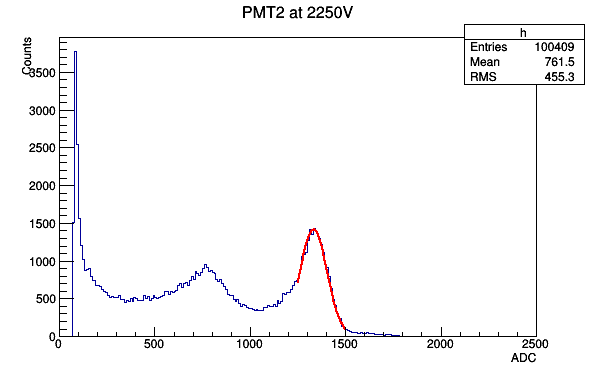
\includegraphics[scale=0.39]{PMT2_2250V.png}
\centering
\caption{Spectrum of the Bismuth source for the PMT1 (PMT2) operating at the high voltage of  2200 V (2250 V), with the second Bismuth peak fitted with a Gaussian, obtaining the mean value of 885 (1334) ADC.}
\label{fig:pmt_fits}
\end{figure}

Therefore the linear relation energy vs ADC for each PMT is given respectively by

\begin{equation}
    E_1 (\MeV) = 0.0013 \cdot {\rm ADC} - 0.058,
\end{equation}

\begin{equation}
    E_2 (\MeV) = 0.00081 \cdot {\rm ADC} - 0.024.
\end{equation}

\newpage

\section{The foil}

The foil used in this experiment is made of iron or aluminium (38 mm x 100 mm x 10 $\mu$m). Iron is a ferromagnetic material. It exhibits a strong magnetism in the same direction of the field, when a magnetic field is applied to it. Due to this characteristic we can study the coincidence as a function of its polarisation. Aluminium cannot be polarised, therefore it is used to prove that the experiment is unbiased.\\

The foil is placed between the radioactive source and the PMTs. The support for the foil is a metallic frame with two coils (Figure \ref{fig:cible}), which will allow the polarisation. The whole structure is fixed inside the enclosure. In order to measure the longitudinal polarisation of $\beta$ particles, target electrons should be polarised in the direction of incident electrons. Therefore, the foil is tilted with an angle of 30 degrees, allowing a longitudinal component of the polarisation, as illustrated in Figure~\ref{fig:30}.

\begin{figure}[H]
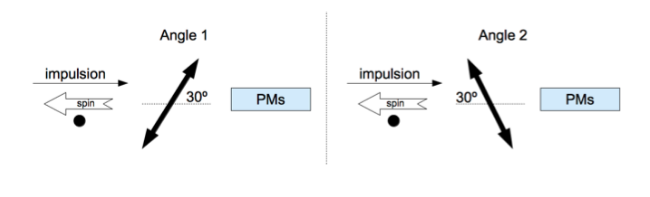
\includegraphics[scale=0.5]{Foil30.png}
\centering
\caption{Schematic of the two possible orientations of the foil}
\label{fig:30}
\end{figure}

In order to estimate the systematic errors due to possible asymmetries in the setup (in particular the effect of the magnetic field and the differences between the two PMTs), the foil will be placed in two different directions as shown in Figure~\ref{fig:cible}. \\

Moreover, we reverse the magnetic field every 5 minutes, since we reverse the direction of the current in the coils. In this way, the polarisation changes, which helps us to reach the goal of the experiment. That goal is to measure the number of electrons detected with polarisation up and with polarisation down, and check if it exists any asymmetry between them.

\subsection{Polarisation of the foil}\label{polfoil}

The aim of this section is to estimate the polarisation of the foil using its hysteresis cycle. To polarise the foil we use an internal coil (red coils in Figure \ref{fig:cible}). It is connected to a signal generator, which provides a 2.7 kHz alternate signal. This signal induces a magnetic field in an external coil, placed around the foil. The induced current passes through a RC circuit (Figure \ref{fig:int}). In this circuit $\omega >>1/RC$, since $R = 10^4 \pm 5\%$ $\Omega$ and $ C = 10^{-6} \pm 20\%$ F, thus the circuit works as an integrator. 

\begin{figure}[H]
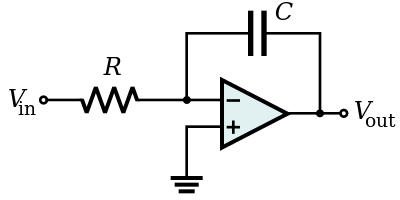
\includegraphics[scale=0.3]{integrator.png}
\centering
\caption{Diagram of the integrator.}
\label{fig:int}
\end{figure}

To simplify the calculations, we assume that the circuit is an ideal one, which means that the impedance is infinite. Therefore, the current in the capacitor is 

\begin{equation}
    I_C = C \frac{dV_C}{dt}.
\end{equation}

Since $I_{\rm out}=I_{\rm in}$, $V_C = V_{\rm out}$ and knowing the Ohm law

\begin{equation}
    \Delta V_{\rm out}= \frac{1}{R C} \int V_{\rm in} dt,
\end{equation}

and by also using the Faraday-Neumann-Lenz law, we finally obtain
\begin{equation}
    \Delta V_{out}= \frac{1}{R C} \Delta \phi, 
\end{equation}

where $\phi$ is the flux crossing the coil, $\phi = B \cdot N \cdot S$, $B$ is the magnetic field, N is the number of turns in the coil (N=1000), and S is the area of the surface (S=$ 0.4 \pm 0.01\  {\rm mm}^2$). \\

The hysteresis curve on the oscilloscope is illustrated in Figure~\ref{fig:curve}. From it we can extract the value of the tension, $\Delta V_{\rm out} = 0.06/2 = 3 \cdot 10^{-2}\  {\rm V}$.

\begin{figure}[H]
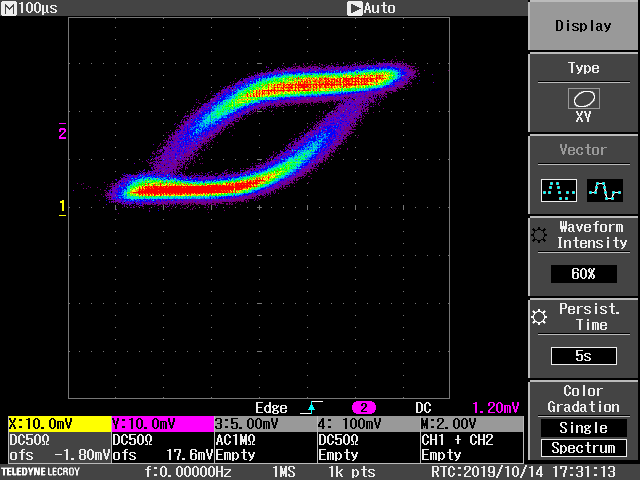
\includegraphics[scale=0.3]{SCRN0004.PNG}
\centering
\caption{Hysteresis curve of the iron foil.}
\label{fig:curve}
\end{figure}

The saturation magnetic field is given by
\begin{equation}
    B = \frac{C \ R \ \Delta V_{\rm out}}{N \ S}.
\end{equation}

Computing the central value by the formula above and the error with the formula for the error propagation, we obtain the saturation magnetic field to be 

\begin{equation*}
    \mathbf{B = (0.75 \pm 0.3)\ T}.
\end{equation*}

The magnetic field and the magnetisation of the foil are related by the following relation: $B = \mu_0 (H+M)$, where the vacuum permeability is $\mu_0 = 4 \pi \cdot 10^{-7}\  {\rm TmA}^{-1}$. The relation can be approximated by $B \approx \mu_0 M$, because of the ferromagnetic properties of the iron.\\

The polarised electron fraction (f) is related with the magnetisation as

\begin{equation}
    f = \frac{M}{\mu_B \rho} = \frac{B}{\mu_B \mu_0 \rho},
\end{equation}

where the Bohr magneton is $\mu_B = 9.27 \cdot 10^{-24} \ {\rm JT}^{-1}$, and $\rho$ is the polarised electrons density. Since only the external electrons contribute to the magnetisation (2 electron per atom), and we can compute easily the number of iron atoms, we obtain $\rho = (1.69 \pm 0.02) \cdot 10^{-30} \ e^-{\rm m}^{-3}$. Putting all together and using the formula for the propagation of uncertainty for the total error, we obtain the polarised electron fraction to be

\begin{equation*}
    \mathbf{f = (3.8 \pm 1.14)\%}.
\end{equation*}

\chapter{Data analysis}
\label{chapter:DataAnalysis}

\section{Analysis}

As we explained in the previous Section \ref{asym}, we want to verify the parity violation of the weak interaction, which has a vector-axial nature. We need to measure the count rate of the asymmetry with the Equations \ref{27} and \ref{30}. We can modify the last equation in such a way that the variable will be the number of events detected

\begin{equation}\label{30}
\epsilon=\frac{C_{\rightleftarrows}-C_{\leftleftarrows}}{C_{\rightleftarrows}+C_{\leftleftarrows}}.
\end{equation}

%\begin{equation}\label{epsi}
%   \epsilon = \frac{N_{\rm up}-N_{\rm down}}{N_{\rm up}+N_{\rm down}} .
%\end{equation}

The data have been divided in five independent data sets. The first three of them have been taken with the orientation of the foil as shown in the left part of the Figure~\ref{fig:30}, the remaining data set, with the opposite orientation.\\

First of all, we need to determine the energy range accessible in the experiment. Since the PMTs are placed at an angle of $35\pm 11 ^o$, only the electrons with a range of energies from 0.2 \MeV~up tp 2.3 \MeV, are detected in the PMT. But in Figure~\ref{fig:up}, where the spectrum of the energy for the polarisation up is shown for PMT1, we notice there is also a peak around zero. It is the background, or PMT noise, that we have evaluated in the previous chapter. 

\begin{figure}[H]
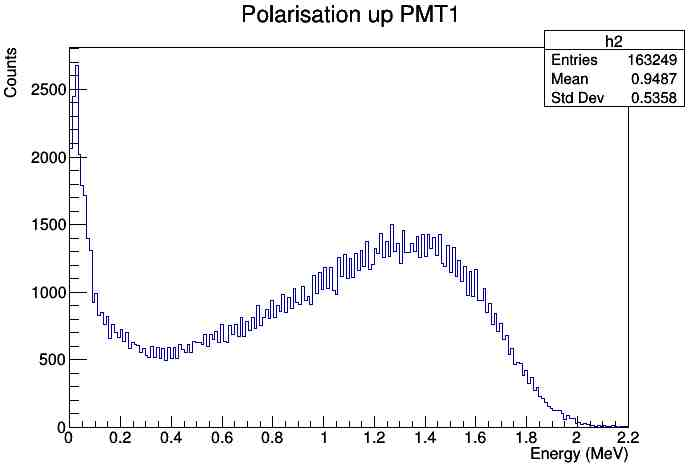
\includegraphics[scale=0.3]{upPMT1.jpg}
\centering
\caption{Spectrum energy for polarisation up for the PMT1.}
\label{fig:up}
\end{figure}

In order to improve the quality of the analysis, the absolute value of the energy difference for each PMT is required to be less than 0.4 \MeV, as illustrated in Figure \ref{fig:PMT1_cut}, for the foil polarisation up (left) and down (right). We can also observe that the energy value for the maximum count of electrons is higher for the polarisation up than for the polarisation down. However, the number of electrons detected for the down polarisation is higher than the number detected for the up polarisation.

\begin{figure}[H]
\begin{subfigure}{.5\textwidth}
  \centering
  % include first image
  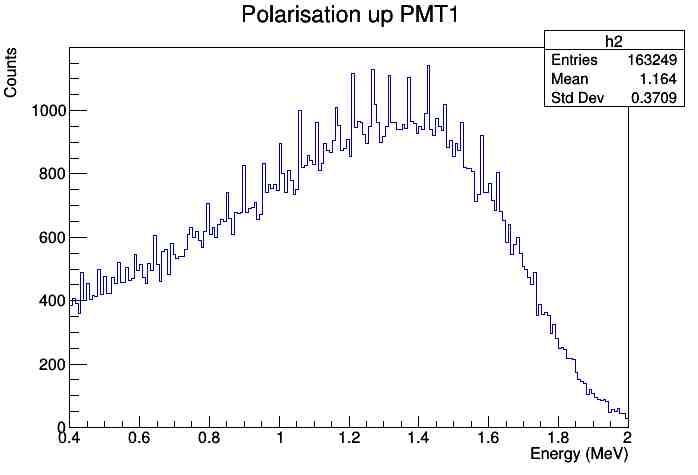
\includegraphics[width=.98\linewidth]{upPMT1cut.jpg}  
  \caption{Polarisation up for PMT1 for energies [0.4-2.0] \MeV.}
\end{subfigure}
\begin{subfigure}{.5\textwidth}
  \centering
  % include second image
  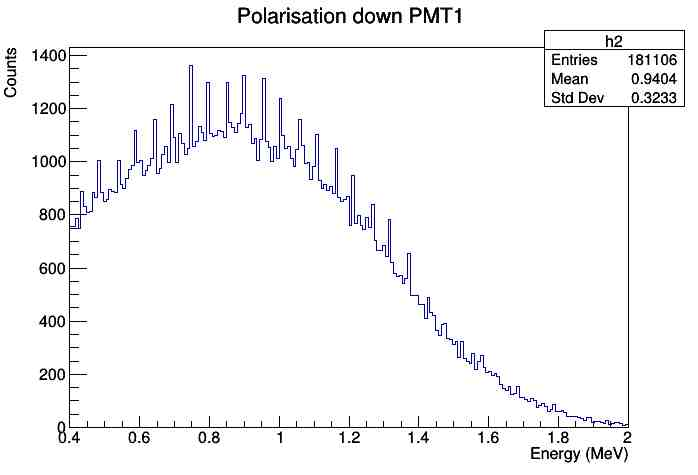
\includegraphics[width=.99\linewidth]{downPMT1cut.jpg}  
  \caption{Polarisation down for PMT1 for energies [0.4-2.0] \MeV.}
\end{subfigure}
\caption{Count of electrons vs energy for PMT1, with an energy selection between 0.4 \MeV~and 2.0 \MeV, for foil polarisation up (left) and down (right).}
\label{fig:PMT1_cut}
\end{figure}

In Figures \ref{fig:Poldown} and Figure \ref{fig:Polup}, it is shown the 2D plots of the coincidences as a function of the energy in both PMTs. We can see that there is a difference in the number of detection depending on the polarisation applied. %It is part of a systematic error. The magnetic field that deviates the electrons and their trajectories are favoured by one of the PMT. This is not a problem, since this preference changes with the polarisation, therefore, we can consider it null in average.

\begin{figure}[H]
\begin{subfigure}{.5\textwidth}
  \centering
  % include first image
  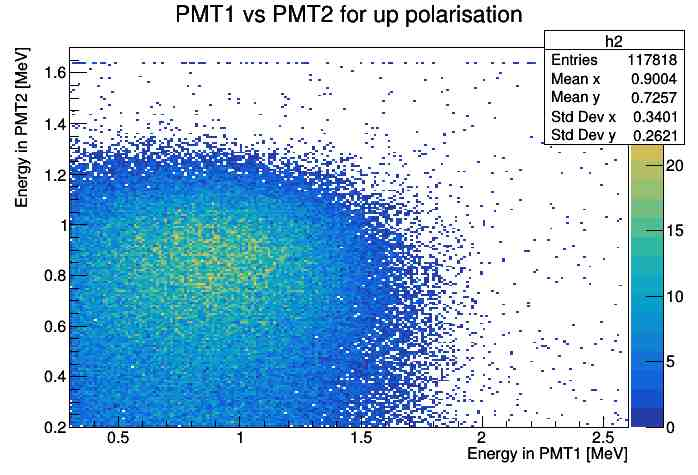
\includegraphics[width=.99\linewidth]{UPPolX.jpg}  
  \caption{Coincidence distribution for the up polarisation.}
  \label{fig:Polup}
\end{subfigure}
\begin{subfigure}{.5\textwidth}
  \centering
  % include second image
  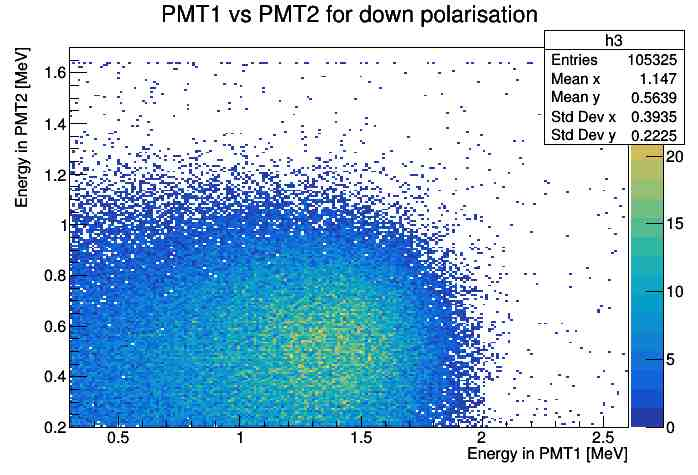
\includegraphics[width=.99\linewidth]{downPolX.jpg}  
  \caption{Coincidence distribution for the down polarisation.}
  \label{fig:Poldown}
\end{subfigure}
\caption{2D distributions of the coincidences versus the energies of both PMTs for the Iron foil.}
\label{fig:fig}
\end{figure}

In Figures \ref{fig:unup} and \ref{fig:undown} we can see the distributions of the coincidence as a function of the energy in both PMTs of the Aluminium foil. As expected, the two distributions are very similar.

\begin{figure}[H]
\begin{subfigure}{.5\textwidth}
  \centering
  % include first image
  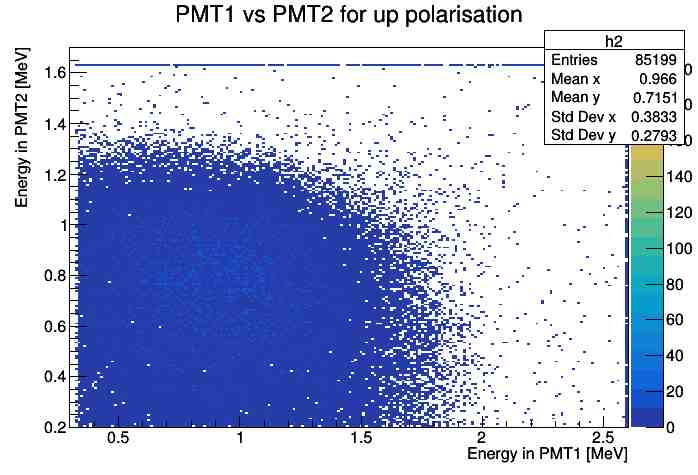
\includegraphics[width=.8\linewidth]{unpolup.jpg}  
  \caption{Coincidence distribution for up polarisation.}
  \label{fig:unup}
\end{subfigure}
\begin{subfigure}{.5\textwidth}
  \centering
  % include second image
  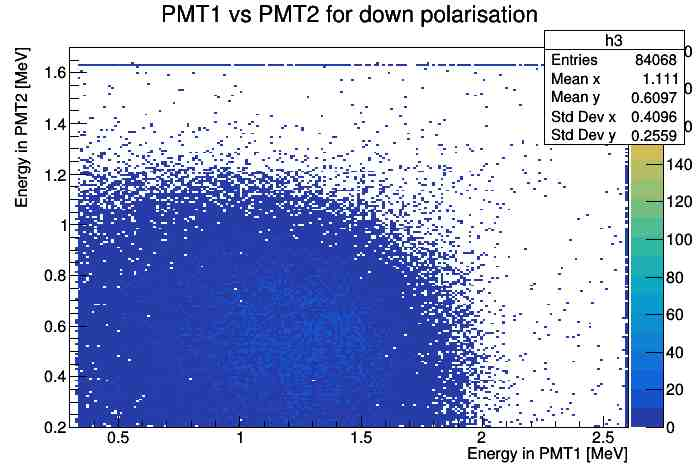
\includegraphics[width=.8\linewidth]{unPoldown.jpg}  
  \caption{Coincidence distribution for down polarisation.}
  \label{fig:undown}
\end{subfigure}
\caption{2D distributions of the coincidences versus the energies of both PMTs for the Aluminium foil.}
\label{fig:unpol}
\end{figure}

\section{Results}

\subsection{Asymmetry}

With the Formula~\ref{epsi} and the measurements done, we can compute the asymmetry. We made a cut in the data, in order to only take into account the values for the coincidence with energies above 0.4 \MeV. The figure \ref{fig:asymfit} shows the value of the asymmetry for the different data sets we analysed. The asymmetry for the different data sets have been extrapolated with a constant function. The statistical uncertainty has been taken from the fit and the systematic uncertainty has been estimated as the difference between the two values of the fit. 

\begin{figure}[H]
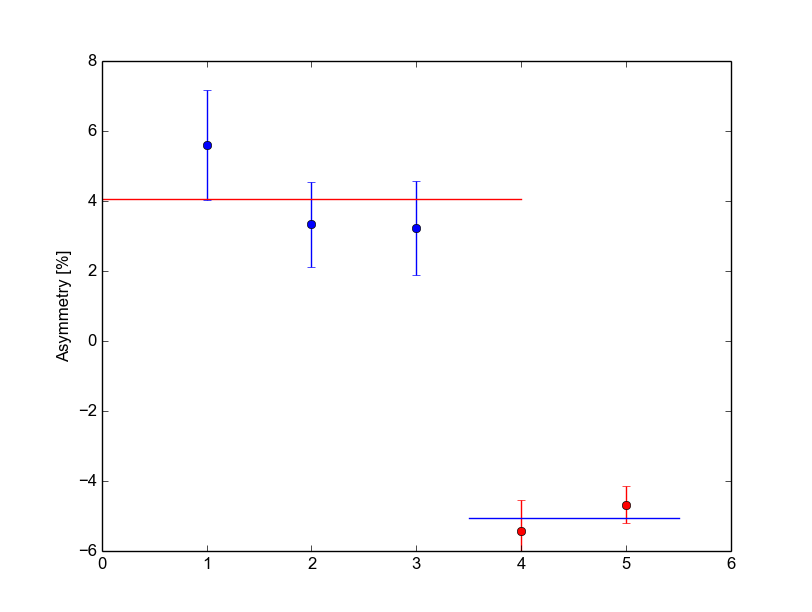
\includegraphics[scale=0.25]{epsilon.png}
\centering
\caption{Value of the asymmetry for different data sets, fitted to a constant function.}
\label{fig:asymfit}
\end{figure}

The final result is 

\begin{equation*}
    \mathbf{\epsilon = (4.56 \pm 0.92 ({\rm stat.}) \pm 0.5 ({\rm sys.}))\%}.
\end{equation*}

We can see that the asymmetry is different from zero, therefore, therefore we have confirmed a parity violation in the weak interactions.\\

Using the same formula, we can compute the asymmetry for the Aluminium foil as

\begin{equation*}
    \mathbf{\epsilon = (0.6 \pm 0.43 ({\rm stat.}))\%}.
\end{equation*}

In this case, we cannot estimate the systematic error since we only used one orientation of the foil. For the statistical uncertainty, we use the same idea as before. It comes from the fit (average between two points). We can conclude with this result that is compatible with zero. Therefore, there is no asymmetry observed for aluminium, as it is not polarised, as expected. So this it confirms the parity violation observed only for the polarised iron foil, as expected.

\subsection{Polarisation} 

Once that the parity violation has been demonstrated, it is possible to compute the polarisation of the decay electrons.\\

We remind the Equation~\ref{30} discussed in section~\ref{asym}, 

\begin{equation}\label{30}
\epsilon=\frac{C_{\rightleftarrows}-C_{\leftleftarrows}}{C_{\rightleftarrows}+C_{\leftleftarrows}} \approxeq P_{\rm s}  \cdot  P_{\rm t}  \cdot \frac{\sigma_{\rightleftarrows}-\sigma_{\leftleftarrows}}{\sigma_{\rightleftarrows}+\sigma_{\leftleftarrows}}= P_{\rm s} \cdot P_{\rm t} \cdot A(\theta,\beta),
\end{equation}

where $P_{\rm s}$ is the longitudinal polarisation of the electrons emitted by the source and $P_{\rm t}$, the longitudinal polarisation of the electrons in the target. Since the foil is tilted by 30 degrees, $P_{\rm t} = f\cdot \cos(30^o)$. As a consequence we obtain the following relation:

\begin{equation}\label{Ps}
    P_{\rm s} = \frac{\epsilon}{f \cdot \cos(30^o) \cdot A(\theta, \beta)}.
\end{equation}

Equation \ref{Ps} is true for a single energy, scattering angle, and angle between the trajectory of the electron and the foil. The problem of averaging the expression is, in general, very complicated. It is simplified if the accept energy range is reasonably narrow. In particular, we consider $A(\theta, \beta)=1$ because the diffusion angle is $\theta = \pi/2$ and the electron do not have a relativistic speed.\\

The polarisation of the target, $f=(3.8 \pm 1.14)\%$, computed in Section~\ref{polfoil}, gives us the final result for the polarisation as

\begin{equation*}
    \mathbf{ P_{\rm s} = (137 \pm 33 ({\rm foil}) \pm 2 ({\rm sys.}))\%},
\end{equation*}

where the error called foil is due to the propagation errors where we also take into account the error on the asymmetry, and the systematic error is computed for the different values of the asymmetry observed.


\chapter{Conclusion}
\label{chapter:Conclusion}

In conclusion, within the experimental errors (systematics, statistic and foil), the asymmetry is measured to be different than zero, thus confirming the theory predicting parity violation in the weak interaction. Once this is confirmed, the polarisation of the target electrons is measured. The values obtained in this experiment are presented the Table~\ref{tab:summary}.

\begin{table}[H]
    \centering
    \begin{tabular}{|c |c|}
    \hline
         $\mathbf{B [T]}$ & $\mathbf{0.75 \pm 0.3}$ \\
         \hline
         $\mathbf{f [\%]}$ & $\mathbf{3.8 \pm 1.14}$\\
         \hline
         $\mathbf{\epsilon [\%]}$ & $\mathbf{4.56 \pm 0.92 (stat) \pm 0.5 (sys)}$\\
         \hline
        $\mathbf{P_{\rm s} [\%]}$ & $\mathbf{137 \pm 33(foil) \pm 2(sys)}$\\ 
        \hline
    \end{tabular}
    \caption{Summary of values measured.}
    \label{tab:summary}
\end{table}

The main source of error arises from the polarisation of the foil. The second largest uncertainty associated to the measurement comes from the magnetic field (Subsection \ref{polfoil}). A flux-meter could be used to improve the measurement of the magnetic flux with and without the foil, and the difference between these two measurement will give the foil contribution.\\



\pagebreak


% Adding a bibliography if citations are used in the report
\bibliographystyle{plain}
\bibliography{BiBTeXexempel.bib}
\begin{thebibliography}{}
\bibitem{}
http://dpnc.unige.ch/~bravar/PPA2/PPA2-L10.pdf

\bibitem{}
http://dpnc.unige.ch/~bravar/PPA2/PPA2-L9.pdf
\bibitem{}
http://dpnc.unige.ch/~bravar/PPA2/PPA2-L8.pdf
\bibitem{}
http://dpnc.unige.ch/~bravar/PPA2/PPA2-L7.pdf
\bibitem{}
 Modern particle physics - Thomson, Mark 
 \bibitem{}
 A Modern Introduction to Quantum. Field Theory. Michele Maggiore
 \bibitem{}
 http://archive.is/NhDVF
 \bibitem{}
 http://archive.is/NhDVF\#selection-777.0-777.36
 \bibitem{}
 https://ocw.mit.edu/courses/physics/8-01sc-classical-mechanics-fall-2016/readings/MIT8\_01F16\_chapter15.pdf
 \bibitem{}
 http://www.radioactivity.eu.com/site/pages/Strontium\_90.htm
 \bibitem{}
 https://www.sciencedirect.com/topics/physics-and-astronomy/photomultiplier-tubes
 \bibitem{}
 https://www.bipm.org/cc/CIPM/Allowed/96/CIPM09\_Materials\_WG\_Report\_Part\_2.pdf
 \bibitem{}
  Determination of Electron and Positron Helicity with Moller and Bhabha Scat- tering,J.D. Ullman et al
  \bibitem{violation}
    Robert Novick.Thirty Years Since Parity Nonconservation, A Symposium for T.D. Lee. Bri-khäuser, 1988.
    \bibitem{paritos}
    H. Frauenfelder, A. O. Hanson, N. Levine, A. Rossi, and G. DePasquali.Phys. Rev. 107 643
    \bibitem{parity}
    T. D. Lee and C. N. Yang.Phys. Rev. 104 254.
 \end{thebibliography}
% Adds reference to the Bibliography in the ToC
\addcontentsline{toc}{chapter}{\bibname}


\end{document}

